\chapter{From Vectors to Tensors} \label{ch:vectors}

\section{What we need to unlearn}

We are first introduced to vectors in two different yet closely related and simplified forms. We're now going to rethink them as an abstraction, which will require us to be careful not to depend on any intuitions derived from our earlier encounters.

That's not to say that we will be abandoning the schoolhouse version of vectors; rather, we will be properly placing them in the context of a more general framework. Also they will very often help ground us, as long as we recognise their limitations.

\subsection{Arrows with direction and length}

The first way to think of vectors is by visualising them as arrows that have a direction and a length. Two vectors $\vec{a}$ and $\vec{b}$ can be added (Figure \ref{fig:vector-addition}) by laying them head to tail, so the sum $\vec{c}$ is the vector starting at the tail of $\vec{a}$ and ending at the head of $\vec{b}$.

\begin{figure}[h]
    \centering
    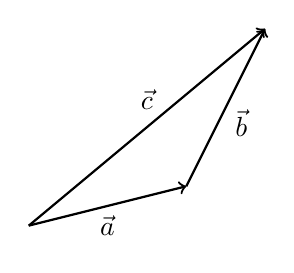
\begin{tikzpicture}        
        \draw[thick,->] (0,0) -- (2,0.5);
        \node at (1,0) {$\vec{a}$};
        \draw[thick,->] (2,0.5) -- (3,2.5);
        \node at (2.7,1.3) {$\vec{b}$};
        \draw[thick,->] (0,0) -- (3,2.5);
        \node at (1.5,1.6) {$\vec{c}$};
    \end{tikzpicture}
    \caption{Adding arrows.} \label{fig:vector-addition}
\end{figure}

Scaling a vector (multiplying it by a number) just alters its length without changing its direction, e.g. multiply by $0.5$ to shrink the vector to half its prior length.

We also learn about the dot product, a scalar-valued operator between two vectors, $\vec{p}\cdot\vec{q}$. If the two vectors $\vec{p}$ and $\vec{q}$ are separated by angle $\theta$, and we know the magnitude (length) of each vector, e.g. $\|\vec{p}\|$, then:

$$
\vec{p}\cdot\vec{q} = \|\vec{p}\| \|\vec{q}\|\cos{\theta}
$$

When we get onto the abstract definition of a vector it may seem like the geometric viewpoint has been relegated to a special case, less fundamental. But it is often useful to keep it in your mind as a way to visualise vectors of any kind, because however abstractly they are defined, they will always be closely analogous to the familiar arrows.

\subsection{Columns of numbers}

The second concrete way to think of vectors is as columns of ordinary numbers, and the number of \textit{dimensions} of the space tells us how many numbers a column vector has to contain. In this form, to add two vectors we just deal with the rows separately: add the numbers in row $1$, and then the numbers in row $2$ and so on for however many rows there are in a column vector, and thus obtain the sum as a column:

$$
\begin{bmatrix}2 \\ 0.5\end{bmatrix} +
\begin{bmatrix}1 \\ 2\end{bmatrix} =
\begin{bmatrix}3 \\ 2.5\end{bmatrix}
$$

More succinctly we can use index notation $a_n$ to mean the value in the $n$th row of the column associated with vector $\vec{a}$, so to add two vectors we just do this:

$$
a_n + b_n = c_n
$$

Scaling a vector just involves multiplying all the rows by the same number:

$$
d_n = x a_n
$$

The dot product is extremely simple in this representation: like with addition, you treat each row separately, multiplying the numbers in row $1$ and so on, but then you just sum all the products to get the numeric value:

$$
\sum_n a_n b_n
$$

\subsection{Coordinates}

These two perspectives are united by introducing a coordinate grid (Figure \ref{fig:vector-coordinate-grid}).

\begin{figure}[h]
    \centering
    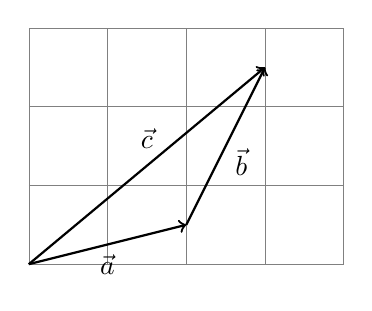
\begin{tikzpicture}       
        \draw[step=1cm,gray,very thin] (0,0) grid (4,3); 
        \draw[thick,->] (0,0) -- (2,0.5);
        \node at (1,0) {$\vec{a}$};
        \draw[thick,->] (2,0.5) -- (3,2.5);
        \node at (2.7,1.3) {$\vec{b}$};
        \draw[thick,->] (0,0) -- (3,2.5);
        \node at (1.5,1.6) {$\vec{c}$};
    \end{tikzpicture}
    \caption{Coordinate grid.} \label{fig:vector-coordinate-grid}
\end{figure}

Much of this subject is concerned with ensuring that our choice of coordinate grid doesn't get confused with the physical facts. We're trying to get answers about nature, and those answers better not change just because we used a different coordinate grid. One of the most important ideas in physics is that vectors are primarily geometric objects. They can be described with numeric coordinates, but there is no preferred coordinate basis. A vector has an independent existence, because it describes something in the physical world.

But however abstract things get, it can often be helpful to remember that you can visualise vectors as arrows and think of the basic operations on them geometrically, and equally it can be helpful to remember that we will always have a way of representing vectors as columns of numbers (indeed, columns of numbers \textit{are} vectors.)

The primary intuition we've been implicitly relying on so far is \textit{orthonormality}. With arrow vectors we can simply see when they are orthogonal, or to be more precise we can measure the angle between vectors, and we can measure their lengths, and we can choose a unit length, and so on. We can simply draw a unit vector, and then draw another unit vector that is orthogonal to it.

Likewise from the column vectors we have no difficult choosing a set of orthonormal vectors, the \textit{standard basis}. They are \textit{one-hot}, all values zero except for a single $1$. In an $n$-dimensional space there can only be $n$ such distinct vectors.

None of these intuitive leaps will be available with abstract vector spaces, and orthonormality cannot be used as an elemental building block. We will build a quite rich set of more fundamental concepts before we invent orthonormality.

By the way, when in physics we speak of a \textit{vector field}, that is, a vector at each point in space, such as wind speed and direction, or the electric field, we visualise arrows spread out over space. But the value of the field in two different places may be the same.

This is obvious (and less confusing) in the case of a scalar field, such as temperature. At two different locations in a room, the temperature may be the same. It's a numerical value that varies from place to place, and the same number may appear in two places.

But exactly the same is true for a vector field. If the wind is some particular speed and direction at two different places on the map, we say the vectors are equal: they are the \textit{same vector}. From the point of view of considering their equality, it is irrelevant that they are associated with different locations in physical space. In vector space, there is one vector with that direction and length.\footnote{Although it will turn out that the luxury of using the same vector space for every point in physical space is only afforded to us if we assume that physical space is flat, which we will for now.}

On to the abstract stuff.

\section{Vectors as elements of a vector space}\label{sec:vectors-space}

A vector space is a set of objects, called vectors, about which we assume nothing except that we can perform certain operations on them.

\subsection{They can be added}

There is an operator $+$ that takes two objects from the set and returns another from the same set (we say it's a \textit{closed} operator).

This operator is commutative:

$$\vec{u} + \vec{v} = \vec{v} + \vec{u}$$

and associative:

$$\vec{u} + (\vec{v} + \vec{w}) = (\vec{v} + \vec{u}) + \vec{w}$$

There is a special object called $0$ (the \textit{zero vector}), which makes no difference when added to any object from the set:

$$\vec{v} + 0 = \vec{v}$$

Also every object has an opposite, known as its additive inverse, so they pair up. The inverse of $\vec{v}$ is written as $-\vec{v}$, and:

$$\vec{v} + (-\vec{v}) = 0$$

The above can written as $\vec{v} - \vec{v}$. Evidently $0$ is its own inverse.

Referring back to schoolhouse vectors, we can see how the arrows and the columns have an addition operation that satisfies all these requirements.

\subsection{They can be scaled}

For any vector space we must nominate an associated set of objects called scalars, having its own abstract requirements. In classical physics we almost always use the real numbers $\mathbb{R}$ as the scalars (in QM we use the complex numbers $\mathbb{C}$).

Our vectors can be multiplied by a scalar to get another object. Scaling them by $1$ makes no difference. Scaling them by $-1$ discovers the additive inverse.

Given two scalars $a$ and $b$, we can compute $c = ab$ and then scale an object $\vec{v}$ by it, or we can separately scale the object first by $a$ and then by $b$, and the result is the same:

$$(ab)\vec{v} = a(b\vec{v})$$

Scaling is distributive over addition of objects:

$$a(\vec{u} + \vec{v}) = a\vec{u} + a\vec{v}$$

And also over addition of scalars:

$$(a + b)\vec{v} = a\vec{v} + b\vec{v}$$

Again, arrows and columns have no problem meeting these requirements.

\subsection{Other Examples of Vector Spaces}

Any set of objects for which we can define these operations is a vector space, not just arrows and columns. The set of ordered tuples of real numbers $\mathbb{R}^n$ is just the column vectors with $n$ rows each. Also there is no reason why $n$ shouldn't be $1$, which means that the plain old set of real numbers $\mathbb{R}$ is also vector space. Think of the real number line as My First Vector Space\texttrademark.

Also the complex numbers $\mathbb{C}$, and tuples of them $\mathbb{C}^n$, work just as well. The example of $\mathbb{C}$ as a vector space is particularly interesting because of its close similarly to $\mathbb{R}^2$. The major difference is that it has a definition of multiplication as a closed operation over its vectors (such that the product of two vectors is a vector), which is absolutely not a general feature of vector spaces.\footnote{Although it is also defined (very differently) in $\mathbb{R}^3$ as the cross product, $\times$.}

In quantum mechanics we will contend with infinite-dimensional complex vector spaces.

\subsection{Fields}

The kind of set that can serve as a scalar is called by mathematicians a \textit{field} (an unfortunate collision of terminology given the very different meaning in physics), which is a set of objects on which we have defined addition, subtraction, multiplication and division, so real or complex numbers usually serve this purpose (and always do in physics), but vectors in general cannot serve as a field of scalars for other vector spaces, because the definition of a vector space says nothing about there being a natural way to multiply or divide pairs of vectors to obtain other vectors.

In the same way, you can't have a vector space of $\mathbb{R}$ over the field of $\mathbb{C}$, because although we can use regular multiplication to "scale" a vector from $\mathbb{R}$ by a scalar from $\mathbb{C}$, the result is likely to be a member of $\mathbb{C}$ but not of $\mathbb{R}$, and thus not a vector from the same space.

Unless we say otherwise, we'll assume the field is $\mathbb{R}$.

\subsection{Finding a Basis}

If we select two vectors $\vec{a}$ and $\vec{b}$ from the space, we may find that they only differ by a scalar ratio $x$:

$$
\vec{a} = x \vec{b}
$$

If there is an $x$ that can scale $\vec{b}$ into $\vec{a}$ then those two vector are \textit{colinear}\footnote{This literally means "on the same line". Note the interesting use of geometrical language, even though we're not supposed to be thinking about arrows in this abstract discussion} (we are careful not to say they point in the same direction because if $x$ is negative then they point in exactly opposite directions, but are still colinear.)

But if there is no such $x$ then they are not colinear. This gives them an interesting superpower:

$$
\vec{r} = x \vec{a} + y \vec{b}
$$

By varying the scalar coefficients $x$ and $y$ we can construct any vector $\vec{r}$ in a two-dimensional \textit{subspace} of the vector space.

We can generalise on this idea a bit by rearranging the equation (and supposing that $x$ becomes negative). If for two vectors $\vec{a}$ and $\vec{b}$ we can find a scalar ${x}$ so that:

$$ 
\vec{a} + x \vec{b} = 0
$$

then they are colinear. Suppose the two vectors point in the same direction but $\vec{a}$ is twice the length of $\vec{b}$. Then we can set $x = -2$ and the sum will cancel out. This is only possible because they are colinear. If it's not possible, we've found a pair of \textit{linearly independent} vectors. Now we can look for a third:

$$ 
\vec{a} + x \vec{b} + y \vec{c} \ne 0
$$

Supposing we find such a vector $\vec{c}$ for which there is no scalar $y$ that satisfies the above equation, then we have found three linearly independent vectors. Or to put it another way, it is not possible to make $\vec{c}$ by any weighted sum of $\vec{a}$ and $\vec{b}$:

$$
\vec{c} \ne x \vec{a} + y \vec{b}
$$

Visualising geometrically, we could say that $\vec{c}$ points outside of the planar subspace reachable by linear combination of $\vec{a}$ and $\vec{b}$. Now we can construct any vector in three dimensions:

$$
\vec{r} = x \vec{a} + y \vec{b} + z \vec{c}
$$

Eventually we may find (assuming the space is finite dimensional) that it is not possible to extend our linearly independent set $\vec{a}, \vec{b}, \vec{c}, ...$ any further. The size of this set tells us how many dimensions the space has, and these vectors are said to \textit{span} the space.

The vitally important thing to realise about this is that at no point have we said that these vectors are orthogonal. We haven't even defined what that means yet. We've only defined the property of linear independence. Nevertheless we have arrived at the idea of a coordinate grid; it's just that our grid may be awkwardly slanted, made of identical parallelogram tiles rather than identical square tiles.

So we don't have to keep choosing letters, we will label each dimension with an integer.\footnote{Note that this use of integers is quite wasteful, as usually they can be added, multiplied, etc. but we will just be using integers as mere labels.} The set of linearly independent vectors that we can use to construct any other vector in the space is called a \textit{basis}. The basis vectors are traditionally written as $\vec{e}_n$, where $n$ is often 1-based (although in Relativity it may be 0-based; this is purely a notational convention and makes no arithmetic difference). The scalar coefficients, which we will call coordinates, that construct a given vector $\vec{r}$ can also be numbered, conventionally with superscript $r^n$:

\begin{equation}
\begin{split}
\vec{r} &= r^1 \vec{e}_1 + r^2 \vec{e}_2 + ... + r^n \vec{e}_n \\
        &= \sum_n r^n \vec{e}_n
\end{split}
\end{equation}

The use of a superscript index is obviously asking for trouble given that it looks like we're raising $r$ to a power\footnote{or possibly indicating an undetermined footnote?}, but this notation is universal in physics so we may as well get used to it.

Having chosen a basis, we can describe any vector with a tuple of coordinates $r^n$, so any vector space of dimension $N$ whose scalar field is $\mathbb{F}$ must be isomorphic with $\mathbb{F}^N$. In other words, all vectors can be described by column vectors, but the numbers in the columns will depend on our choice of basis.

But the laws of physics cannot possibly care what basis we choose, so we need ways of obtaining numeric facts about vectors that do not depend on the choice of basis.

\section{Covectors} \label{covector}

Think of a scalar-valued function of a vector. That is, a black box with a single input slot accepting a vector $\vec{a}$, and an output hole that gives us back a scalar $x$ (Figure \ref{fig:1-slot-box}).

\begin{figure}[h]
    \centering
    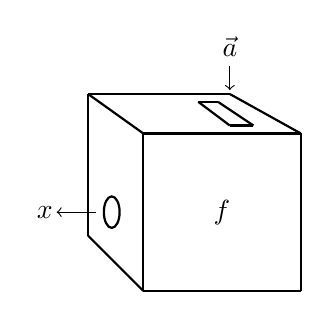
\begin{tikzpicture}
        \draw[thick] (0,0) -- (2,0);
        \draw[thick] (2,0) -- (2,2);
        \draw[thick] (2,2) -- (0,2);
        \draw[thick] (0,2) -- (0,0);
        \draw[thick] (0,2) -- (-0.7,2.5);
        \draw[thick] (-0.7,2.5) -- (-0.7,0.7);
        \draw[thick] (-0.7,0.7) -- (0,0);
        \draw[thick] (-0.7,2.5) -- (1.1,2.5);
        \draw[thick] (1.1,2.5) -- (2,2);

        \draw[thick] (1.4,2.1) -- (0.95,2.4);
        \draw[thick] (0.95,2.4) -- (0.7,2.4);
        \draw[thick] (0.7,2.4) -- (1.1,2.1);
        \draw[thick] (1.1,2.1) -- (1.4,2.1);
        
        \node at (1.1,3.1) { $\vec{a}$};
        \draw[->] (1.1,2.85) -- (1.1,2.55);

        \node at (-1.25,1) { $x$};
        \draw[thick] (-0.4,1) ellipse (0.1 and 0.2);
        \draw[->] (-0.6,1) -- (-1.1,1);

        \node at (1,1) { $f$};

    \end{tikzpicture}
    \caption{Function $f$ with a single slot accepting a vector} \label{fig:1-slot-box}
\end{figure}

More precisely, this machine is a mapping from the vector space to the real numbers. There are infinitely many such mappings and they could be arbitrarily complicated. We will restrict ourselves to a simple subset of these mappings.

First, we note that it is possible to define the addition operator on mappings:

$$
f(\vec{a}) = g(\vec{a}) + h(\vec{a})
$$

That is, it could be that inside the box $f$, there are concealed two boxes $g$ and $h$. When $f$ receives an input vector $\vec{a}$, it passes it to both $g$ and $h$, and adds their results together to obtain its own result. Note that we haven't yet restricted the complexity of $g$ and $h$; we have no idea what they do to produce their individual results.

Likewise, it is possible to scale a mapping by a factor $x$:

$$
f(\vec{a}) = x g(\vec{a})
$$

The trick to restricting the complexity of our set of possible mappings is to require that they comply with the rules of a vector space. Not only can they be added and scaled, but combinations of these operations produce consistent results. But if we do that, then we have also ensured that the set of allowed mappings actually \textit{is} a vector space. Every mapping we care about must be a vector chosen from that space.

Note that we haven't proven that every possible mapping is a vector. We've merely restricted ourselves to only considering a subset of mappings, those that can be scaled and added to find other mappings from the same restricted subset, such that scaling a mapping by 5 is the same as scaling that mapping by 2 and separately by 3 and then adding those two scaled mappings.

If we label the original vector space $V$ then this associated vector space of mappings $V \mapsto \mathbb{R}$ is written as $V^*$ and is called the dual space of $V$. All we've discovered so far about $V$ also applies to $V^*$, including the idea of a set of mappings being linearly independent, which means we can select a basis of mappings chosen from $V^*$ and thus construct any mapping from it by scaling and adding the basis mappings. That's quite a leap, so pause to digest it. The moment you discover a set of objects is a vector space, you know you can choose a basis, and then describe anything in that space in terms of a weighted sum of that basis.

We call the mappings taken from $V^*$ \textit{covectors}. The basis covectors are labelled with superscripts $\vec{e}^n$ and the coordinates with subscripts $f_n$, so we can build any covector from the chosen basis:

\begin{equation}
    \begin{split}
    \vec{f} &= f_1 \vec{e}^1 + f_2 \vec{e}^2 + ... + f_n \vec{e}^n \\
            &= \sum_n f_n \vec{e}^n
    \end{split}
\end{equation}

It follows that, just as $N$-dimensional vectors are isomorphic with columns of $N$ scalars, so too are their associated covectors.

It is sometimes suggested that all vector spaces have a dual space, as if this was some property hiding in the definition of a vector space. But in truth we have conjured the dual space into existence, first by inventing the idea of a mapping $V \mapsto \mathbb{R}$, then by defining operations on those mappings, then by considering the set of all possible mappings, and finally by imposing the rules of vector spaces, which restricts us to a subset of the possible mappings that we named covectors. There is nothing particularly automatic about this. We made it happen by being curious about ways in which vectors might be mapped to scalars.

Another important point to note is that as covectors are vectors, the operation we've been writing as $f(\vec{a})$ is in fact much more symmetrical than that notation implies. We combine a vector from $V$ and a covector from $V^*$ and this produces a scalar from $\mathbb{R}$. 

So we could equally say that a vector "operates" on a covector to produce the scalar. From the point of view of $V^*$ it is $V$ that is the dual space. There is a more symmetrical notation\footnote{Unfortunately there is almost no consistency on notation in this topic; we're just picking one of many possible notations for this.} we can use to make this clear:

$$\langle \vec{f},\vec{a}\rangle$$

In this notation, the left and right sides of the operation are from mutually dual spaces, mirror opposites that annihilate one another leaving only a scalar residue.

Although we will mostly think of a covector as a function and a vector as something that can be a parameter to a covector, keep in mind that just as we've thought of a covector as machine that accepts a vector as input, we could just as well think of a vector as a machine that accepts a covector as input.

\subsection{Connecting the Dual Spaces}

We obviously have a lot of freedom when choosing a basis in either $V$ or $V^*$. What can we usefully do to relate the two sides? We've seen how a covector may be built as a weighted sum of basis covectors $\vec{e}^i$ from $V^*$:

$$
\vec{f} = \sum_i f_i \vec{e}^i
$$

And likewise a vector is built as a weighted sum of basis vectors $\vec{e}_i$ from $V$:

$$
\vec{v} = \sum_i v^i \vec{e}_i
$$

If we have the vector $\vec{v}$ and we want to extract its $i$th coordinate, $v^i$, that's a function from a vector in $V$ to a scalar, that is, it's a covector from $V^*$. We could choose the basis covectors so that the $i$th basis covector extracts the $i$th coordinate of the vector passed to it:

$$
v^i = \langle \vec{e}^i , \vec{v} \rangle
$$ 

Equivalently, if we have a covector $\vec{f}$ and we want to extract its $j$th coordinate, $f_j$, then we need to pass $f$ an input vector chosen from $V$, and we could choose the basis vectors so that the $j$th basis vector makes $\vec{f}$ produce the $j$th coordinate of $\vec{f}$:

$$
f_j = \langle \vec{f} , \vec{e}_j\rangle
$$

It doesn't matter which of those two ways we approach this, because either will constrain the other. We can substitute $\vec{f}$ expressed as a sum:

$$
f_j = \langle \sum_i f_i \vec{e}^i , \vec{e}_j\rangle
$$

and linearity allows us to separately deal with each dimension and sum their results:

$$
f_j = \sum_i f_i \langle \vec{e}^i , \vec{e}_j\rangle
$$

But if that's true for \textit{any} $\vec{f}$, and not just a coincidence applying to some specific example, then the scalar factor $\langle \vec{e}^i , \vec{e}_j\rangle$ must be "selecting" just one of the $f_i$ terms, specifically the one where $i = j$, and eliminating all others, or to put it more succinctly using the Kronecker delta (§\ref{def:Kronecker}):

$$
f_j = \sum_i f_i \delta \indices{^i_j}
$$

So if the $f_j$ are indeed the components of the covector, discovered by making it act on the basis vectors, we've discovered the relationship that must exist between the dual bases:

\begin{equation}
    \langle \vec{e}^i,\vec{e}_j\rangle = \delta\indices{^i_j}
    \label{eqn:dual-bases-delta}
\end{equation}

So we could choose any basis at all in $V$, and then definition \eqref{eqn:dual-bases-delta} restricts the choice of basis in $V^*$, or vice versa. Such is the symmetry of this situation, we could instead have let a basis covector $\vec{e}^j$ act on a randomly chosen vector $\vec{a}$ and require that this give us the $j$th coordinate of $\vec{a}$, and we'd have reached the same conclusion.

From now on we'll assume that this alignment of the dual bases has been performed. That being the case, we can compute the action of a covector on a vector by arithmetic on their coordinates:

\begin{equation}
    \begin{split}
        \langle \vec{f},\vec{a}\rangle 
        &= \langle \sum_i f_i \vec{e}^i , \sum_j a^j \vec{e}_j \rangle \\
        &= \sum_{ij} f_i a^j \langle\vec{e}^i,\vec{e}_j\rangle \\
        &= \sum_{i} f_i a^i
    \end{split}
\end{equation}

So the linearity allows us to sum over all combinations of $i, j$ and pull the coordinates outside of the action of the covector on the vector, and the dual bases yield the value $1$ where $i = j$ and $0$ otherwise, so we just end up with a simple sum over the products of the paired-up coordinates.

In a roundabout way we've discovered the dot product, albeit between a covector and a vector rather than two ordinary vectors. We still haven't introduced any concept of orthonormality, or even orthogonality, between pairs of vectors. Our "coordinate grid" is still not necessarily a lattice of squares, and our dot product is between elements of two different (dual) vector spaces, but we always choose their basis vectors so they are related by a definite requirement, which we can state in two ways:

\begin{enumerate}
    \item The $n$th basis covector from $V^*$ can be used to extract the $n$th coordinate of a vector from $V$.
    \item The $n$th basis vector from $V$ can be used to extract the $n$th coordinate of a covector from $V^*$.
\end{enumerate}

And as a consequence of this (dual) requirement we find that when the $n$th basis covector acts on the $m$th basis vector, the result is $1$ if $m = n$ and $0$ if $m \ne n$.

If we describe our covectors and vectors as sets of coordinates, to make a covector act on a vector we simply perform the dot product between their coordinates. Or equivalently, we write the covector as a single row matrix on the left, and the vector as a single column matrix on the right, and perform matrix multiplication to get a single scalar.

Does this mean we've created a dual link between \textit{every} vector and a corresponding covector? Absolutely not. We've only linked up the basis vectors with the basis covectors. Still, there is an obvious mapping between vectors and covectors: let the covector have exactly the same coordinates as its vector pair, $f_i = v^i$. And indeed this is the assumption made with schoolhouse vectors, where we freely perform the dot product between vectors described by coordinates, without worrying about whether they are from mutually dual spaces.

But that is only one possible mapping out of an infinity of possibilities, as we could blend the coordinates by any weighted sum we like. So connecting the basis covectors with the basis vectors is a start, but still leaves something to be desired.

\subsection{Visualising the dual basis} \label{sec:dual-bases}

It may be worth pausing here to see how this result relates to our schoolhouse version of arrows and coordinates and the dot product. In that world-view, the coordinates are just the scaling factors that weight the orthonormal basis vectors to construct a vector, and the dot product of a basis vector $\vec{e}_i$ and a given vector $\vec{a}$ produces the $a_i$ coordinate of $\vec{a}$. This is how we understand the geometric dot product (with $\cos \theta$) to be related to the idea of simply plucking one of the numbers from a column vector.

But what happens if we deny all knowledge of orthogonality? If we choose any linearly independent basis vectors (Figure \ref{fig:vectors-non-orth-1}) we can still sum them to generate any vector in the space (Figure \ref{fig:vectors-non-orth-2}).

\begin{figure}[h]
    \caption{Building a vector from any basis}
    \begin{subfigure}{0.5\textwidth}
        \centering
        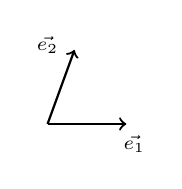
\begin{tikzpicture}
            \node at (1.1,-0.25) {\scriptsize $\vec{e_1}$};
            \draw[thick,->] (0,0) -- (0.342,0.940);
            \node at (0,1) {\scriptsize $\vec{e_2}$};
            \draw[thick,->] (0,0) -- (1,0);
        \end{tikzpicture}
    \caption{Any old basis $\vec{e}_n$} \label{fig:vectors-non-orth-1}
    \end{subfigure}
    \begin{subfigure}{0.5\textwidth}
        \centering
        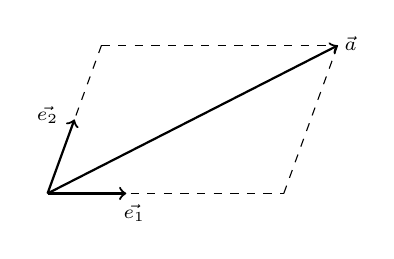
\begin{tikzpicture}
            \draw[dashed] (0,0) -- (3,0);
            \draw[dashed] (3,0) -- (3.684,1.879);
            \draw[dashed] (0,0) -- (0.684,1.879);
            \draw[dashed] (0.684,1.879) -- (3.684,1.879);
            \node at (1.1,-0.25) {\scriptsize $\vec{e_1}$};
            \draw[thick,->] (0,0) -- (0.342,0.940);
            \node at (0,1) {\scriptsize $\vec{e_2}$};
            \draw[thick,->] (0,0) -- (1,0);                    
            \draw[thick,->] (0,0) -- (3.684,1.879);
            \node at (3.85,1.9) {\scriptsize $\vec{a}$};
        \end{tikzpicture}
        \caption{$\vec{a} = a^1 \vec{e}_1 + a^2 \vec{e}_2$} \label{fig:vectors-non-orth-2}
    \end{subfigure}
\end{figure}

The problem comes when we try to recover the coordinates by projecting $\vec{a}$ onto the two basis vectors (Figure \ref{fig:vectors-non-orth-3}).

\begin{figure}[h]
    \caption{Projecting a vector onto a carelessly chosen basis}
    \begin{subfigure}{0.5\textwidth}
        \centering
        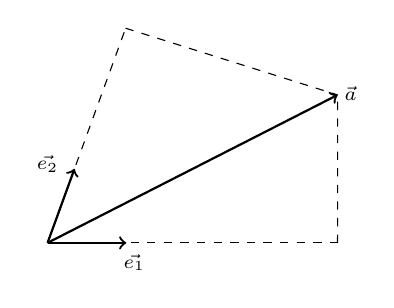
\begin{tikzpicture}
            \draw[dashed] (0,0) -- (3.684,0);
            \draw[dashed] (3.683,0) -- (3.684,1.879);
            \draw[dashed] (0,0) -- (0.992,2.726);
            \draw[dashed] (0.992,2.726) -- (3.684,1.879);
            \node at (1.1,-0.25) {\scriptsize $\vec{e_1}$};
            \draw[thick,->] (0,0) -- (0.342,0.940);
            \node at (0,1) {\scriptsize $\vec{e_2}$};
            \draw[thick,->] (0,0) -- (1,0);                    
            \draw[thick,->] (0,0) -- (3.684,1.879);
            \node at (3.85,1.9) {\scriptsize $\vec{a}$};
        \end{tikzpicture}
    \caption{Projecting $\vec{a}$ back onto the basis} \label{fig:vectors-non-orth-3}
    \end{subfigure}
    \begin{subfigure}{0.5\textwidth}
        \centering
        \begin{tikzpicture}
            \draw[dashed] (0,0) -- (3.684,-1.339);
            \draw[dashed] (3.683,-1.339) -- (3.684,1.879);
            \draw[dashed] (0,0) -- (0,3.218);
            \draw[dashed] (0,3.218) -- (3.684,1.879);
            \node at (1.2,-0.20) {\scriptsize $\vec{e^1}$};
            \draw[thick,->] (0,0) -- (0,1);
            \node at (-0.2,1.2) {\scriptsize $\vec{e^2}$};
            \draw[thick,->] (0,0) -- (0.992,-0.342);                    
            \draw[thick,->] (0,0) -- (3.684,1.879);
            \node at (3.85,1.9) {\scriptsize $\vec{a}$};
        \end{tikzpicture}
        \caption{$\vec{a} = a_1 \vec{e^1} + a_2 \vec{e^2}$} \label{fig:vectors-non-orth-4}
    \end{subfigure}
\end{figure}

We can visualise this projection process by drawing lines from the tip of $\vec{a}$ so they meet at right angles with the lines extended from the basis vectors. But these imply different coordinates for $\vec{a}$ from the ones that we used to build it using the basis $\vec{e}_n$.

This raises the question: in what basis are these the coordinates for $\vec{a}$? There is such a basis (Figure \ref{fig:vectors-non-orth-4}), $\vec{e^n}$, and we label the coordinates with subscripts, $a_n$, so the reconstructed $\vec{a}$ is given by:

$$
\vec{a} = a_1 \vec{e^1} + a_2 \vec{e^2}
$$

This basis $\vec{e}^j$ is related to the original basis $\vec{e}_i$ by \eqref{eqn:dual-bases-delta}. Looking at it geometrically (that is, cheating), when choosing the dual basis vector for a given index, we must choose a vector that is visibly orthogonal to all the other basis vectors, and this means we will have a severely limited choice, because there can be only one alignment that meets this requirement. Furthermore the magnitude of the vector $\vec{e}^i$ is fully determined by the requirement that $\langle \vec{e}_i, \vec{e}^i \rangle = 1$, as the ratio between the coordinates is already fixed by the choice of alignment.

In this visualisation process we have shown the relationship between $V$ and $V*$ by overlaying them on the same diagram, but they are in fact separate vector spaces: elements of $V$ are not elements of $V*$, and vice versa. But the way we have calibrated these two sets of bases to be mutually consistent is exactly the same as the relationship between the bases of $V$ and $V*$.

If the original basis vectors had been orthogonal, the dot product would have produced exactly the same coordinates we'd used to build the vector in the first place, i.e. figures \ref{fig:vectors-non-orth-2}, \ref{fig:vectors-non-orth-3} and \ref{fig:vectors-non-orth-4} would all be identical: a rectangle with the vector as its diagonal. But of course, we haven't yet said precisely what orthogonality means.

\subsection{The same ideas in coordinates}

We can make this concrete by playing with $\mathbb{R}^2$ as our vector space $V$, in which case the dual space of covectors $V^*$ contains mappings $\mathbb{R}^2 \mapsto \mathbb{R}$.

\begin{figure}[h]
    \caption{Basis vectors in $\mathbb{R}^2$}
    \begin{subfigure}{0.5\textwidth}
        \centering
        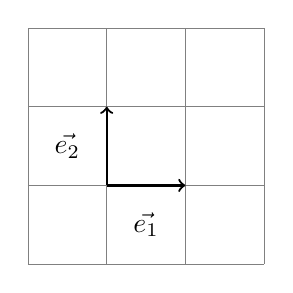
\begin{tikzpicture}
            \draw[step=1cm,gray,very thin] (1,1) grid (4,4); 
            \draw[thick,->] (2,2) -- (3,2);
            \node at (2.5,1.5) {$\vec{e_1}$};
            \draw[thick,->] (2,2) -- (2,3);
            \node at (1.5,2.5) {$\vec{e_2}$};        
        \end{tikzpicture}
        \caption{Orthonormality} \label{fig:vectors-orthonormality}
    \end{subfigure}
    \begin{subfigure}{0.5\textwidth}
        \centering
        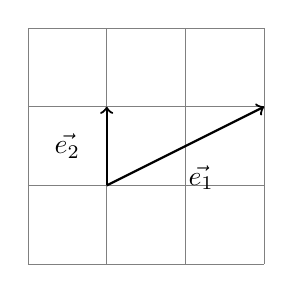
\begin{tikzpicture}
            \draw[step=1cm,gray,very thin] (1,1) grid (4,4); 
            \draw[thick,->] (2,2) -- (4,3);
            \node at (3.2,2.1) {$\vec{e_1}$};
            \draw[thick,->] (2,2) -- (2,3);
            \node at (1.5,2.5) {$\vec{e_2}$};
        \end{tikzpicture}
        \caption{Awkwardness} \label{fig:vectors-awkwardness}
    \end{subfigure}
\end{figure}

With our schoolhouse foreknowledge it would be easy to choose an orthonormal basis in $\mathbb{R}^2$ (Figure \ref{fig:vectors-orthonormality}):

$$
\vec{e}_1 = \begin{bmatrix}1 \\ 0\end{bmatrix}\,,\,
\vec{e}_2 = \begin{bmatrix}0 \\ 1\end{bmatrix}
$$

But we still haven't defined what orthonormal means, so we'll just choose something awkward (Figure \ref{fig:vectors-awkwardness}):

$$
\vec{e}_1 = \begin{bmatrix}2 \\ 1\end{bmatrix}\,,\,
\vec{e}_2 = \begin{bmatrix}0 \\ 1\end{bmatrix}
$$

By the way, it is customary to put the basis vectors in a row matrix, $\begin{bmatrix}\vec{e}_1 & \vec{e}_2\end{bmatrix}$, so they can be matrix-multiplied by a column representation of a vector in $V$, but that's not what we're doing here. We are giving the definition of each basis vector as a matrix, and the basis vectors are ordinary vectors belonging to $V$, and customarily they are presented as column matrices.

What is the corresponding $V^*$ basis, $\vec{e}^i$? It has to obey:

$$
\langle \vec{e}_j,\vec{e}^i \rangle = \delta_{ij}
$$

Some straightforward equation building and substitution yields:

$$
\vec{e}^1 = \begin{bmatrix}0.5 & 0\end{bmatrix}\,,\,
\vec{e}^2 = \begin{bmatrix}-0.5 & 1\end{bmatrix}
$$

And these being covectors from $V^*$, we present them as row matrices. Using our $V$ basis we can construct a vector $\vec{v}$ from the coordinates $(2, 3)$:

$$
\vec{v} = 2\vec{e}_1 + 3\vec{e}_2
        = \begin{bmatrix}4 \\ 2\end{bmatrix} + \begin{bmatrix}0 \\ 3\end{bmatrix} 
        = \begin{bmatrix}4 \\ 5\end{bmatrix}
$$

What happens if we evaluate the $V^*$ basis covectors against $\vec{v}$?

$$
\begin{bmatrix}0.5 & 0\end{bmatrix} \begin{bmatrix}4 \\ 5\end{bmatrix} = 2 
\,,\,
\begin{bmatrix}-0.5 & 1\end{bmatrix} \begin{bmatrix}4 \\ 5\end{bmatrix} = 3
$$

We get back the correct coordinates. If we'd just transposed the $V$ basis vectors into rows and left-multiplied them, we would have obtained wrong answers: this is precisely the same problem we saw with projecting onto the non-orthogonal basis.

But the utility of these basis covectors is limited to their ability to extract a scalar coordinate from a vector. For example, there is nothing here that generally relates any vector (other than the basis vectors) with a specific covector partner, or anything that relates one vector with another.

\section{Tensors}

Let's upgrade our black box machine so it has two input slots, accepting vectors $\vec{a}$ and $\vec{b}$ from the same vector space $V$, but still one output hole that gives us back a scalar $x$ (Figure \ref{fig:2-slot-box}).

\begin{figure}[h]
    \centering
    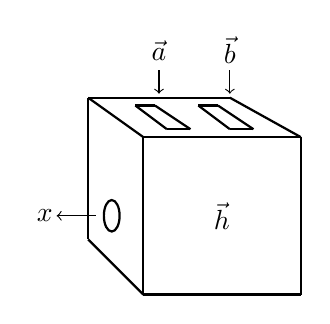
\begin{tikzpicture}
        \draw[thick] (0,0) -- (2,0);
        \draw[thick] (2,0) -- (2,2);
        \draw[thick] (2,2) -- (0,2);
        \draw[thick] (0,2) -- (0,0);
        \draw[thick] (0,2) -- (-0.7,2.5);
        \draw[thick] (-0.7,2.5) -- (-0.7,0.7);
        \draw[thick] (-0.7,0.7) -- (0,0);
        \draw[thick] (-0.7,2.5) -- (1.1,2.5);
        \draw[thick] (1.1,2.5) -- (2,2);

        \draw[thick] (1.4,2.1) -- (0.95,2.4);
        \draw[thick] (0.95,2.4) -- (0.7,2.4);
        \draw[thick] (0.7,2.4) -- (1.1,2.1);
        \draw[thick] (1.1,2.1) -- (1.4,2.1);

        \draw[thick] (0.6,2.1) -- (0.15,2.4);
        \draw[thick] (0.15,2.4) -- (-0.1,2.4);
        \draw[thick] (-0.1,2.4) -- (0.3,2.1);
        \draw[thick] (0.3,2.1) -- (0.6,2.1);
        
        \node at (0.2,3.1) { $\vec{a}$};
        \draw[->] (0.2,2.85) -- (0.2,2.55);

        \node at (1.1,3.1) { $\vec{b}$};
        \draw[->] (1.1,2.85) -- (1.1,2.55);

        \node at (-1.25,1) { $x$};
        \draw[thick] (-0.4,1) ellipse (0.1 and 0.2);
        \draw[->] (-0.6,1) -- (-1.1,1);

        \node at (1,1) { $\vec{h}$};

    \end{tikzpicture}
    \caption{Box $\vec{h}$ with two slots accepting vectors} \label{fig:2-slot-box}
\end{figure}

This is a mapping from pairs of vectors to scalars: $V \times V \mapsto \mathbb{R}$.

Suppose \textit{only to begin with} that the machine had an especially simple inner mechanism: inside the box $\vec{h}$, there are two single-slot boxes (covectors) $\vec{f}$ and $\vec{g}$. The machinery inserts input $\vec{a}$ into box $\vec{f}$, and input $\vec{b}$ into box $\vec{g}$, to obtain two scalars, which it simply multiplies together to produce its own resultant scalar that falls out of the hole of $\vec{h}$. In other words, it's really just two covectors glued together by scalar multiplication, and they act independently on the inputs:

$$
h(\vec{a}, \vec{b}) = \langle \vec{f},\vec{a} \rangle \langle \vec{g},\vec{b} \rangle
$$

In fact this design only accounts for a subset of the machines, but it will serve as an intuitive building block for us to construct all the machines we're interested in. We can write it as $\vec{f} \otimes \vec{g}$, which is called the \textit{tensor product} of the two covectors.

So sticking with this simplified design to begin with, consider the space of all such machines containing two covectors. We can define addition and scaling on these pairs in a way that satisfies the requirements of a vector space. Addition is easy. Much as we defined addition for covectors by simply adding their results when given the same input vector, we'll add these two-slot machines by adding their results when they act on the same pair of vectors:

\begin{equation}
\begin{split}
    (\vec{f} \otimes \vec{g} + \vec{p} \otimes \vec{q})(\vec{a}, \vec{b}) 
    &= 
    \vec{f} \otimes \vec{g} (\vec{a}, \vec{b}) + \vec{p} \otimes \vec{q}(\vec{a}, \vec{b}) \\
    &= \langle \vec{f}, \vec{a} \rangle
        \langle \vec{g}, \vec{b} \rangle
    + \langle \vec{p}, \vec{a} \rangle
        \langle \vec{q}, \vec{b} \rangle    
\end{split}        
\end{equation}

Scaling by some $x$ is even easier:

$$
\left[x(\vec{f} \otimes \vec{g})\right](\vec{a}, \vec{b}) 
= x(\vec{f} \otimes \vec{g})(\vec{a}, \vec{b}) 
= x \langle \vec{f}, \vec{a} \rangle
    \langle \vec{g}, \vec{b} \rangle
$$
 
Thus we have defined a vector space, and so these two-slot machines are also vectors. We can form a basis for that space by taking all possible pairs of basis covectors, $\vec{e}^i \times \vec{e}^j$. If the (co)vector space is $N$-dimensional, the pair-space will be $N^2$-dimensional, because it requires $N^2$ basis machines to span the space. Any two-slot machine can therefore be written as a linear combination (a weighted sum) of all the basis machines:

$$
\sum_{ij} M_{ij} (\vec{e}^i \otimes \vec{e}^j)
$$

And therefore to describe any two-slot machine in terms of the basis we will need $N^2$ numbers, which we can write as $M_{ij}$. By the way, there's no pressing need to think of it as a matrix, although we sometimes do. The $M$ stands for "machine" in this case. It's just a list of $N^2$ numbers, labelled with two indices that each can take on $N$ integer values, supplying the weighting for each basis machine.

Inserting two vectors $\vec{a}$ and $\vec{b}$ into the slots just means:

$$
\sum_{ij} M_{ij} \langle \vec{e}^i,\vec{a} \rangle \langle \vec{e}^j,\vec{b} \rangle
$$

Recall that an expression like $\langle \vec{e}^i,\vec{a} \rangle$ is the scalar resulting from $\vec{e}^i$ acting on $\vec{a}$. But as the input vector $\vec{a}$ can be described using the same (dual) basis, $a^k \vec{e}_k$: 

$$
\sum_{ijk} M_{ij} \langle \vec{e}^i, a^k \vec{e}_k \rangle \langle \vec{e}^j,\vec{b} \rangle
$$

and the same for $\vec{b}$:

$$
\sum_{ijkl} M_{ij} \langle \vec{e}^i, a^k \vec{e}_k \rangle \langle \vec{e}^j,b^l \vec{e}_l \rangle
$$

Both these substitutions required us to introduce a new summation index, because we are essentially "multiplying out" between the existing expression's summation terms and those of the vector we are substituting. So if the vector space is $2$-dimensional, the above is summing $2 \times 2 \times 2 \times 2 = 16$ terms. By linearity:

$$
\sum_{ijkl} M_{ij} a^k \langle \vec{e}^i, \vec{e}_k \rangle b^l \langle \vec{e}^j, \vec{e}_l \rangle
$$

We know the basis covectors acting on the basis vectors have very simple results by definition: $\langle \vec{e}^i, \vec{e}_k \rangle$ evaluates to $1$ if $i = k$, but is $0$ otherwise. Likewise $\langle \vec{e}^j, \vec{e}_l \rangle$ is $1$ if $j = l$ but $0$ otherwise. Therefore the $12$ summation terms where either $i \ne k$ or $j \ne l$ must vanish, leaving only $4$ terms where they are equal and the covector-vector interactions are simply replaced with $1$. Therefore we can replace $k$ with $i$ and $l$ with $j$ throughout:

\begin{equation}
    \sum_{ij} M_{ij} a^i b^j
        \label{eqn:two-slot-computation}
\end{equation}

So to compute the scalar result we only need the coordinates of the two input vectors and a list of numeric parameters that fully defines how the machine operates, creating summation terms that contribute various weightings of every possible combination of coordinates from the two vectors.

This kind of machine is called a \textit{tensor}.

It will often be the case that $M_{ij} = M_{ji}$, which is quite a lot of redundancy. But this is necessary to ensure that the machine is symmetrical: switching the inputs around does not affect the result. Of course, a machine doesn't have to be defined that way.

\subsection{Simple tensors} \label{simple-tensor}

We mentioned at the start that the simplified design (the ordinary product of two scalars obtained by two covectors operating separately on one vector input each) is not powerful enough to describe all these machines, even though we used it to define our basis machines. The simplistic machine is defined by a matrix that can be written as:

$$
M_{ij} = f_i g_j
$$

In other words, it can be decomposed into two separate columns of numbers. Such a machine is known as a \textit{decomposable}, \textit{elementary} or just \textit{simple} tensor.

One hint as to why it is so limited is that as $f_i$ and $g_j$ provide $N$ values each for an $N$-dimensional space, that is only $2N$ adjustable parameters, even though $M$ appears to have $N^2$ independent values. So we aren't allowing the full flexibility of which $M$ is capable.

Of course, if $N=2$ then $N^2 = 2N = 4$, but even then, there is a restrictive pattern that applies regardless of the dimensions. Viewing $M_{ij}$ as a matrix, every row (labelled by $i$) would be a scaled version of the numbers in $g_j$, and every column (labelled by $j$) would likewise be a scaled version of the numbers in $f_i$. That is, the rows are all linearly dependent on one another, and so are the columns. This would not be the case if the elements of $M$ were truly independent.\footnote{Can any symmetric matrix be expressed as the product of a row and a column? No. Try to find a row and a column that can be multiplied to produce the identity matrix. The columns are linearly independent, as are the rows.}

There's a subtlety here though: vector addition and scaling operators are meant to be closed. We've proposed a way of defining simple machines, which is a restricted set of objects, and then we've said that scaling and adding simple machines allows us to discover objects that are not in that simple set, which sounds like we're breaking the rules, reaching outside the initial set.

The resolution to this conundrum is that we are dealing with a general set of machines that can be described by the somewhat misleading notation $V^* \otimes V^*$, which we define as not only the simple machines made of any two covectors $f \otimes g$, but also those machines that are \textit{weighted sums} of one or more simple machines. This broader set includes machines that cannot be decomposed into two covectors. We can however choose a basis from the subset that \textit{can} be decomposed, and we do that because it is that subset for which we are able to directly explain how they operate. And from that basis we can build any machine of the form $V^* \otimes V^*$. Covectors (one-slot machines) are the most basic building block, from which we can make simple (two-slot) machines, from which in turn we can make any machines by linear combination of simple machines.

\subsection{Any number of slots}

Another point to note about these two-slot machines is that although here we focused on $V^* \otimes V^*$, we could instead of chosen $V \otimes V$, in which case the simple machine would have consisted of two vectors, and would have acted on two input covectors (recall how the notation $\langle \vec{f}, \vec{a} \rangle = \langle \vec{a}, \vec{f} \rangle$ emphasises symmetry, so we can think of a covector acting on a vector or a vector acting on a covector with no real difference in the result). We can define machines of the form: 

$$
V \otimes V^* \otimes V \otimes \ldots
$$ 

having any number of slots accepting any mixture of vectors and covectors in some specific order. A machine with five slots will be represented by a list of $N^5$ numbers labelled with five indices. The slots that accept vectors (being defined by covectors) will have down indices, and the slots that accept covectors (being defined by vectors) will have up indices. For example, we can say our machine is from the space:

$$
V \otimes V^* \otimes V \otimes V \otimes V^*
$$ 

or we can say it is represented by the numerical parameters:

$$
M\indices{^i_j^k^l_m}
$$

These convey the same information. Sometimes the indexed parameter notation is used as a compact way to describe the structure of the machine, the only downside being that we have to unnecessarily choose symbols for the indices.\footnote{Some authors call this \textit{slot-naming index notation}, others \textit{abstract index notation}.}

\subsection{What is a tensor?}

These machines, which are used to compute a scalar value from some (co)vector inputs, are all tensors, though as we've seen, the space of machines of a given type is also a vector space, so tensors are vectors.

We have proposed creating a five-slot machine $M\indices{^i_j^k^l_m}$, and so it seems entirely proper to treat a 1-slot machine $M_i$ or $M^i$ as part of the same family of objects. We've been calling them covectors and vectors, which is accurate (we had to invent them first in order to build toward tensors), but they are also themselves tensors in this general sense.

Perhaps more surprising, but no less consistent, is the idea that a machine with no slots also belongs to the same family. It's just a scalar value, which can be thought of as a machine that produces a scalar value from \textit{no} inputs.

Sometimes the type of a tensor is written $(u, d)$ where $u$ tells you how many up indices and $d$ tells you how many down indices it has. So a scalar is a $(0, 0)$-tensor, a vector is a $(1, 0)$-tensor, a covector is a $(0, 1)$-tensor, and we will soon encounter practical uses for $(1, 1)$, $(0, 2)$ and $(2, 0)$-tensors, all of which are also elements of vector spaces.

In summary, everything is seemingly an example of everything else, and yet all are different things.

\subsection{Contraction} \label{tensor-contraction}

When we insert a vector or covector into a suitable slot of a machine, we are effectively merging two tensors, by "wiring up" them up so that they share an index variable, which makes that variable disappear due to summation over it.

Starting with a five-slot machine $M\indices{^i_j^k^l_m}$ (which incidentally is a $(3,2)$-tensor), we will insert a covector $a_k$ into the middle slot, resulting in a machine $N$ with four slots (a $(2,2)$-tensor):

$$
N\indices{^i_j^l_m} = \sum_{k} M\indices{^i_j^k^l_m} a_k
$$

The index $k$ effectively disappears. This process is more formally regarded as a two stage process. First, we form the tensor product, which is an object with a separately named index for every index of the two source tensors:

$$
P\indices{^i_j^k^l_m_n} = M\indices{^i_j^k^l_m} a_n
$$

This step doesn't involve any summation. If the vector space is 4-dimensional, $P$ is a list of $4^6 = 4096$ numbers, each being the product of a distinct pair from the $4^5 = 1024$ numbers in $M$ and the $4$ numbers in $a$.

Then we link two of the slots by giving them the same index name and summing over that index (in this case by renaming $n$ to $k$):

$$
N\indices{^i_j^l_m} = \sum_{k} P\indices{^i_j^k^l_m_k}
$$

It's that second step, renaming $n$ to $k$ and summing over $k$, that is the actual contraction. We could then perform two contractions at once on $N$:

$$
x = \sum_{il} N\indices{^i_i^l_l}
$$

Each contraction ties two indices together and eliminates them, so this last double-contraction has eliminated four indices at once, leaving us with a scalar.

\section{Einstein notation}

We have been following a rule where basis vectors are given subscript indices, while vector components are given superscript indices. Then we do the opposite with basis covectors and components. This means that whenever one basis object acts on another:

$$
\langle e^i, e_j \rangle
$$

they always have opposing index positions. This is mirrored exactly by the way components are allowed to be multiplied. We've found that the dot product is only valid between the coordinates of a vector and a covector, so a product like this inside a summation, where we have repeated the same index variable:

$$
a^i b_i
$$

is valid, but neither of these is allowed because they imply a dot product between two vectors or two covectors:

$$
a^i b^i \, , \, a_i b_i
$$

Here's a real example that we'll encounter later:

$$
\sum_{\mu\nu\beta\lambda} g_{\mu\nu} Z\indices{^\mu_\beta} \underline{a}^{\beta} Z\indices{^\nu_\lambda} \underline{b}^{\lambda}
$$

Every single one of the four indices appears in two places, once up and once down, so it's a quadruple contraction, eliminating all the indices and so the result is a scalar. A simpler example shows how index variables are not necessarily introduced by summation:

$$
b^\mu = \sum_{\nu} O\indices{^\mu_\nu} a^\nu
$$

The $\nu$ index is repeated up/down in the way that is characteristic of all summation variables, but $\mu$ is introduced on the left to indicate that the expression computes the value of one component of several that represent a vector (we know it's a vector rather than a covector because the index is up).

From these patterns Einstein deduced something tremendously helpful: it is completely unnecessary to write the summation symbol and state what the summation index variables are! If an expression consisting of indexed quantities multiplied together contains exactly two references to the same index, once up and once down, then that index is a summation index.

$$
g_{\mu\nu} Z\indices{^\mu_\beta} \underline{a}^{\beta} Z\indices{^\nu_\lambda} \underline{b}^{\lambda}
=
\sum_{\mu\nu\beta\lambda} g_{\mu\nu} Z\indices{^\mu_\beta} \underline{a}^{\beta} Z\indices{^\nu_\lambda} \underline{b}^{\lambda}
$$

$$
b^\mu = O\indices{^\mu_\nu} a^\nu = \sum_{\nu} O\indices{^\mu_\nu} a^\nu
$$

This shorthand applies just as well to basis vectors:

$$
\vec{a} = a^i \vec{e}_i = \sum_{i} a^i \vec{e}_i
$$

The recent example of a tensor product cannot be mistaken for an implied summation because there are no repeated indices:

$$
P\indices{^i_j^k^l_m_n} = M\indices{^i_j^k^l_m} a_n
$$
 
Whereas the contraction example unmistakably sums over $k$ alone:

$$
N\indices{^i_j^l_m} = P\indices{^i_j^k^l_m_k}
$$

\section{The Inner Product} \label{inner-product}

The most important necessity for a specific machine of the form $V^* \otimes V^*$ is to at last come up with a way to define orthogonality, and the norm (length) of a vector, and thus orthonormality, but also a specific two-way pairing between every vector and a covector partner.

Nominating one such machine for a given vector space, we can call it the \textit{inner product}, and we say that the combination of the vector space and its inner product is an \textit{inner product space}.

As we've incessantly complained, we have so far had no way to judge whether two vectors are orthogonal to one another, even though we know that for arrows or column vectors there are some intuitive ways to choose orthogonal vectors. In our abstract development of the subject there was no such thing as orthogonal or orthonormal.

The choice of an inner product determines which vectors are mutually orthogonal, and also which are normalised (of unit norm). Importantly, it will also pair every vector with a single dual covector (and vice versa).

The notation $(\vec{a},\vec{b})$ is sometimes used for the inner product, similar to but deliberately distinct from the $\langle \vec{f},\vec{a}\rangle$ notation for the action of a covector on a vector.\footnote{Sadly the meanings of these notations are sometimes switched, and they aren't the only notations used.}

The \textit{squared-norm} of a vector $\vec{a}$ is $(\vec{a},\vec{a})$, so the norm is $\sqrt{(\vec{a},\vec{a})}$. In most situations (Newtonian and Quantum) there is a rule that the norm must be \textit{positive definite}, meaning that it is never negative and is only zero for the zero vector. The exception is just about anything involving Einstein, who favours inner products that break this rule in every way.

As it's a two-slot machine, its coordinate representation can be thought of as a matrix or a list of numbers addressed by two indices, and it is called the \textit{metric}. In General Relativity the metric is usually written as $g$, and its indices are often $\mu$ and $\nu$, so applying it to vectors $\vec{a}$ and $\vec{b}$ will look like this:

$$
(\vec{a},\vec{b}) = \sum_{\mu\nu} g_{\mu\nu} a^\mu b^\nu
$$

Or expressed in matrix multiplication, we put one of the vectors on the left of the matrix, transposed into a row, and one on the right as a column.

$$
(\vec{a}, \vec{b}) =
\begin{bmatrix}
a^1 & a^2 & a^3
\end{bmatrix}
\begin{bmatrix}
g_{11} & g_{12} & g_{13} \\
g_{21} & g_{22} & g_{23} \\
g_{31} & g_{32} & g_{33}
\end{bmatrix}
\begin{bmatrix}
b^1 \\ b^2 \\ b^3
\end{bmatrix}
$$

The central square matrix is always symmetric, $g_{\mu\nu} = g_{\nu\mu}$, so the vector inputs can be switched without affecting the result. The square matrix can multiply with the right column first, or with the left row: the order of operations doesn't matter.

As we will eventually see, this transposition business will wind up being somewhat messier than simply writing down the summations, in which the symmetry is a lot more obvious. This is one reason why it may not be worth thinking of $g$ (or any other two-slot machine) as a matrix.\footnote{Another reason: what if the machine has three or more slots?}

Compare it to the familiar dot product, which would be:

$$
\vec{a} \cdot \vec{b} = \sum_{\mu} a^\mu b^\mu
$$

It's the same row/square/column matrix multiplication except the central square matrix is missing, or equivalently it's the identity matrix:

$$
(\vec{a}, \vec{b}) =
\begin{bmatrix}
a^1 & a^2 & a^3
\end{bmatrix}
\begin{bmatrix}
1 & 0 & 0 \\
0 & 1 & 0 \\
0 & 0 & 1
\end{bmatrix}
\begin{bmatrix}
b^1 \\ b^2 \\ b^3
\end{bmatrix}
$$

So all the times when you obediently used the dot product to operate on two vectors, you were implicitly setting $g$ to be the Kronecker delta (§\ref{def:Kronecker}):

$$
g_{\mu\nu} = \delta_{\mu\nu}
$$

\textit{By definition} if the inner product is represented by $\delta_{\mu\nu}$ then the basis vectors are orthonormal. In other words, the inner product being represented by the identity matrix doesn't really tell us anything about the inner product. It tells us that we've chosen a set of basis vectors so that they are orthonormal according to this space's nominated inner product. It is always possible to do this, regardless of what the inner product happens to be.\footnote{Strictly speaking it is always possible for a finite-dimensional inner product space.}

This means that if we can use a single inner product consistently, we may as well define the basis to be orthonormal according that inner product, which means we will always be able to use the dot product between vectors, and the distinction between vectors and covectors becomes unimportant. We can even define all other multi-slot machines in terms of vectors acting on other vectors (via the inner product). That is, every machine would be of the form $V \otimes V \otimes V \otimes \ldots$, and would accept vectors as inputs. You may wonder if all that care we took to distinguish superscript and subscript indices was a waste of time. Indeed in many contexts, including all Newtonian classical mechanics and quantum mechanics, it is a waste of time.

The exception is General Relativity, where the inner product varies from place to place, becoming a \textit{tensor field}. To describe it, we have to fix the basis somehow, and allow the metric to vary. As a result of this, if you want to understand GR, you need to understand that to get the squared-norm of a vector, you need to get the equivalent covector so it can act on the original vector. But in many other topics, you can just think of the vector acting on itself.

This also means that the previous examples of what we called awkward basis vectors would in fact be orthonormal if we chose a particular inner product.

\subsection{No such thing as awkward}

Starting with the standard basis in column vectors, we could specify this as the inner product:

$$
g_{\mu\nu} = 
\begin{bmatrix}
\frac{1}{2} & -\frac{1}{2} \\
-\frac{1}{2} & 1
\end{bmatrix}
$$

We had to pick \textit{some} basis as a starting point or we would not have had a way to write down the inner product in numerical form. We used the standard basis, which is made of very simple one-hot vectors, but we now know that we must not call those vectors orthonormal.

Now we'll move the goalposts and choose a different set of vectors to be our basis, and they will be our usual awkward choice:

$$
\vec{e}_1 = \begin{bmatrix}2 \\ 1\end{bmatrix}\,,\,
\vec{e}_2 = \begin{bmatrix}0 \\ 1\end{bmatrix}
$$

Let's test our inner product on every possible pairing of these basis vectors:

$$
(\vec{e}_1, \vec{e}_1) =
\begin{bmatrix}
2 & 1
\end{bmatrix}
\begin{bmatrix}
\frac{1}{2} & -\frac{1}{2} \\
-\frac{1}{2} & 1
\end{bmatrix}
\begin{bmatrix}
2 \\ 1
\end{bmatrix}
= 1
$$    

$$
(\vec{e}_1, \vec{e}_2) =
\begin{bmatrix}
2 & 1
\end{bmatrix}
\begin{bmatrix}
\frac{1}{2} & -\frac{1}{2} \\
-\frac{1}{2} & 1
\end{bmatrix}
\begin{bmatrix}
0 \\ 1
\end{bmatrix}
= 0
$$    

$$
(\vec{e}_2, \vec{e}_1) =
\begin{bmatrix}
0 & 1
\end{bmatrix}
\begin{bmatrix}
\frac{1}{2} & -\frac{1}{2} \\
-\frac{1}{2} & 1
\end{bmatrix}
\begin{bmatrix}
2 \\ 1
\end{bmatrix}
= 0
$$    

$$
(\vec{e}_2, \vec{e}_2) =
\begin{bmatrix}
0 & 1
\end{bmatrix}
\begin{bmatrix}
\frac{1}{2} & -\frac{1}{2} \\
-\frac{1}{2} & 1
\end{bmatrix}
\begin{bmatrix}
0 \\ 1
\end{bmatrix}
= 1
$$    

The basis is orthonormal if $(\vec{e}_i, \vec{e}_j) = \delta_{ij}$. Undeniably, these basis vectors are orthonormal. The inner product says so, and who are we to doubt it? Furthermore, the inner product's matrix \textit{when expressed in this basis} is $\delta_{\mu\nu}$.

Every distinct basis provides a different way to describe any vector with coordinates, and likewise any covector. Regardless of the basis they are described in, the result of applying a specific covector to a specific vector will be the same scalar value. That is, the choice of basis is not a fact about the vector space, but merely a way to describe the vectors in it.

Choosing a different inner product (or equivalently a metric) is not like that. In fact a given physical situation may impose a metric and we have to accept it; it's a fact of nature. So there are two possible reasons why the matrix $g_{\mu\nu}$ might change:

\begin{itemize}
    \item a change of basis, which will change the coordinates $a^{\mu}$ and $b^{\nu}$ of the two input vectors, as well as the matrix elements $g_{\mu\nu}$, so as to ensure the scalar result of the inner product $(\vec{a}, \vec{b})$ is unchanged, or
    \item a change of inner product itself, which will not affect the coordinates of anything else, and thus the scalar result of $(\vec{a}, \vec{b})$ may be very different.
\end{itemize}

\subsection{The metric and its inverse}

As always we must be careful not to confuse the coordinate or matrix representation of an object with the object itself. The matrix $g_{\mu\nu}$ is merely a representation in some basis of a machine with two slots awaiting vectors. 

We know that internal to that machine, it may be simple (consisting of two covectors, which are single-slot machines ready to operate on the two vectors inserted into the slots, and whose scalar results will be multiplied to get the result) or, more generally, it may be a linear combination of such simple two-slot machines.

Therefore if a single vector is inserted into the first slot, it will be fed into the first slot of one or more simple two-slot machines, which will all feed that same vector into their first covector. This will produce a set of scaling factors that apply to the second covector of each simple two-slot machine. This is in effect a set of single-slot machines being linearly combined into a single-slot machine (a weighted sum of covectors).

And we are left with a new single-slot machine awaiting another vector before it can produce a final scalar. In general a machine with $S$ slots can be nibbled away at sequentially, feeding in the $S$ inputs one at a time, each step reducing by one the capacity of the resultant machine to accept further inputs, until eventually all we are left with is a scalar result.

So as advertised, as well as providing a meaning for orthonormality, the metric also provides a complete pairing between every vector and a corresponding covector. Provide a single vector input to the metric and you will get back \textit{the} covector that is the dual partner to that vector, according to the metric.

It follows that if we find the inverse matrix to $g_{\mu\nu}$, that will act on a covector to reveal its dual vector. Or speaking abstractly, we can build something like the inner product but for getting a scalar from two covectors $(\vec{p}, \vec{q})$. Again the starting point is the simplest two-slot machine equivalent internally to two vectors $\vec{a}$ and $\vec{b}$. Each input covector is combined with one of the vectors and the two scalar results are multiplied together:

$$
(\vec{p}, \vec{q}) =
\langle \vec{p}, \vec{a} \rangle
\langle \vec{q}, \vec{b} \rangle
$$

And in general we would allow a linear combination of a basis formed from such simple machines, and of course this would have a matrix representation, because we will choose a vector basis $\vec{e}_{\mu}$, which will determine a covector basis $\vec{e}^{\mu}$:

$$
(\vec{p},\vec{q}) = \sum_{\mu\nu} g^{\mu\nu} p_{\mu} q_{\nu} 
$$

So to recap, $g_{\mu\nu}$ can be evaluated in two stages. First it operates on a vector $a^{\mu}$ to produce \textit{something} that is ready to later operate on some second vector $b^{\nu}$ and so finish the job by producing a scalar. That intermediate something, if it can act on a vector to get a scalar, must be a covector, which we could call $a_{\nu}$, as it is \textit{the} dual of the vector $a^{\nu}$. If the basis happens to be orthonormal, the dual vector and covector will have the same coordinates, $a_{\mu} = a^{\mu}$ (because $g_{\mu\nu} = \delta_{\mu\nu}$). But in any case, once the second vector $b^{\nu}$ is eventually available, the scalar is just the contraction $a_{\nu} b^{\nu}$.

And exactly the same is true for $g^{\mu\nu}$, which can operate on a covector $p_{\mu}$ to produce its unique dual vector $p^{\mu}$.

So with reference to the indices being "up" or "down", $g^{\mu\nu}$ is sometimes called the raising operator, because it turns a covector's coordinates (subscript) into vector coordinates (superscript), while $g_{\mu\nu}$ is the lowering operator, working the other way. And described in this way, it is obvious that $g^{\mu\nu}$ undoes the work of $g_{\mu\nu}$, i.e. they are mutually inverse matrices. With our natural bias toward vectors, if $g_{\mu\nu}$ is the metric then $g^{\mu\nu}$ is the \textit{inverse metric}.

When dealing with objects expressed in coordinates we use the convention that vector coordinates are up and covector coordinates are down, and this lets us always take care to ensure that when we sum their products we always pair a vector (up) with a covector (down) using the same index variable. If necessary we can easily raise or lower using the appropriate version of the metric.

\section{Operators}

In this context, an operator $\hat{O}$ is a function that maps from a vector to a vector, $V \mapsto V$. As usual we are particularly interested in linear operators, for which:

$$
\hat{O} \vec{a}
=
\hat{O}\left(\sum_n a^n\vec{e}_n \right)
= 
\sum_n a^n\hat{O}\vec{e}_n
$$

Why? Because to completely characterise the behaviour of such an $\hat{O}$ we only need to know its effect on the $n$ basis vectors, which we can capture in a square matrix.

This is a new kind of geometric object. It has a physical meaning that is entirely independent of the choice of basis, even though the matrix elements will certainly be different depending on the basis. So just as we can speak of the same vector being represented by different columns of coordinates depending on the choice of basis, we can also speak of the same operator being represented by matrices of different elements depending on the choice of basis.

When we label a matrix with indices, $M_{ij}$, we have choice: should they be subscript or superscript? This was straightforward when we introduced the inner product, because we conceived of it as two covectors tied together by multiplication: $V^* \otimes V^*$, and so their coordinate representations must have subscripts, and hence the metric has subscript indices. Likewise the inverse metric is like two vectors, $V \otimes V$, and so has superscript indices.

In both those cases, we found that as well as acting as a mapping from two inputs to a scalar, the same object could map a single input to its dual partner.

Here we want a machine that maps a vector to a vector. As a hunch, consider the set of $V \otimes V^*$ machines. Such a machine will be a linear combination of simple machines made of a vector and a covector, $\vec{a} \otimes \vec{f}$:

\begin{equation}
\hat{O} = \sum_{\mu\nu} O\indices{^\mu_\nu} \left( \vec{e}_\mu \otimes \vec{e}^\nu \right)
\end{equation}

So the operator is represented (in the current basis) by a matrix with one super and one sub index, being the sum of a set of matrices whose elements are the product of a vector coordinate and a covector coordinate. To find the coordinates of the resultant vector $\vec{b}$ obtained from $\hat{O} \vec{a}$:

$$
b^\mu = \sum_{\nu} O\indices{^\mu_\nu} a^\nu
$$

There are some operators that have the same coordinates in all bases. The $0$-matrix, which maps all vectors to the $0$-vector, has all its elements $0$. The identity operator, which has no effect on its input, is $\delta_{\mu\nu}$ in all bases.

A unitary operator is one that is equivalent to a combination of rotation and reflection. One handy fact about such an operator is that if we have its matrix representation (in any basis), we can find the inverse simply by transposing it:

$$
(O^\intercal) O = I
$$

We can think of a vector as pointing in a direction in space, and this being an aspect of its geometrical nature. How can we similarly characterise operators?

\section{Eigenvectors and Eigenvalues}\label{sec:vectors-eigen}

An operator that performs only scaling is isotropic, treating all directions equivalently. We can (in somewhat woolly terms) think of it as sphere-shaped.

But some operators are biased with regard to direction. To characterise the behaviour of an operator we can consider those vectors which are scaled by it without their direction being altered (the scaling may be negative, leaving the vector pointing the opposite direction; as long as the resulting vector is co-linear with the input vector, that's insignificant enough.) Such vectors are called the \textit{eigenvectors} of the operator, and the scaling value associated with each eigenvector is called an \textit{eigenvalue}. Note that the zero vector is not considered a candidate for an eigenvector. It has no direction, making it impossible to say whether the operator has changed its direction. Also it goes from length zero to length zero under any operator, so any scalar could be the eigenvalue, meaning that the eigenvalue is undefined.

For operators that perform a general isotropic scaling, all input vectors are eigenvectors: all inputs get only scaled, and always by the same eigenvalue.

With vectors in the plane, when the operator is a pure rotation, e.g. by a right-angle anti-clockwise:

$$R_A = \begin{bmatrix}0 & -1 \\ 1 & 0\end{bmatrix}$$

or clockwise:

$$R_C = \begin{bmatrix}0 & 1 \\ -1 & 0\end{bmatrix}$$

every vector changes direction by the same angle, and that means there are no eigenvectors.

More interestingly, there are operators for which only some vectors are eigenvectors. In three dimensions the rotation has an axis, along which all vectors are eigenvectors, and any vectors not on that axis are not eigenvectors. Curiously, even though these eigenvectors don't exist in the planar case, we can find \textit{complex} eigenvalues for them by supposing that such eigenvectors exist, which is weird.

Consider a reflection (call it $M$ for mirror):

$$M = \begin{bmatrix}1 & 0 \\ 0 & -1\end{bmatrix}$$

If we take the first coordinate to be horizontal and the second vertical, this flips the input vector to point up rather than down, or vice versa. So it seems that all vectors have their direction changed and are not eigenvectors, but there exceptions: vectors that lie on the horizontal axis and have no vertical component will be unaffected, i.e. they will be eigenvectors with eigenvalue 1. Also vectors that lie on the vertical axis will have their direction changed, but to the exact opposite direction (their alignment does not change), which is the same as being scaled by -1, and so these too are eigenvectors, but with eigenvalue -1.

So within the space of input vectors, there is a subspace (the \textit{eigenspace}) of eigenvectors, and $M$ has an intrinsic orientation, as there is a particular line around which reflection occurs.

We can find the eigenvectors given a matrix representation $M$ of an operator acting on a vector represented by a column matrix $v$. If $v$ is an eigenvector, and $x$ is the corresponding eigenvalue, what we mean by that is:

$$Mv = xv$$

For the vector $v$, multiplying it by the matrix $M$ is the same as multiplying it by the ordinary number $x$. So with trivial algebra:

$$Mv - xv = 0$$

This is fine because $Mv$ and $xv$ are column matrices, and here $0$ is the column matrix filled with zeros.

Pulling out $v$ as a factor (not quite as trivial):

$$(M - xI)v = 0$$

We have to leave behind the identity matrix $I$ in place of $v$ because we need the matrix equivalent of the ordinary number $x$, so we can subtract it from $M$.

Having split it into two factors whose product is zero, we know that either one or both of the factors must be zero. We already realised we aren't interested in the case where $v$ is the zero vector because its eigenvalue will be undefined (it could be anything). So we refuse to accept $0$ as an eigenvector. Therefore $v$ is not the zero vector, and so the matrix $M - xI$ must be such that it is able to transform some non-zero vector $v$ into the zero vector. This means it has no inverse, as there is no way to recover the direction of the original vector if we've sent it to $0$ (the zero vector has no direction, or has all directions, so direction is a meaningless concept for it.)

Restricting ourselves to a two dimensional vector space, one way to picture the effect of a matrix is to think of it acting on a unit square (where the matrix is $2 \times 2$) and asking what the area of the resulting parallelogram will be. If it is not zero, every point in the original square has a unique point in the parallelogram and vice versa: the matrix is invertible. If the area is zero, the points of the original square have been crammed onto a line of $1$ dimension, so we have destroyed the information about where they came from in $2$ dimensions. All input vectors end up pointing in the same direction, and are only distinguished by length. No linear transform will be able to spread them back out into the correct different directions: the matrix is not invertible.

The area of that parallelogram (or in higher dimensions, the volume of an n-parallelepiped) is called the determinant of the matrix, $\det M$. If it's zero, the matrix is not invertible. And therefore, if:

$$\det{(M - xI)} = 0$$

then we definitely have some eigenvalues. The determinant can be expanded out into a polynomial expression in $x$ (there are various methods; a popular one is to get a computer to do it) and then solved by factoring to find all the $x$ values that make one of the factors $0$. We can then plug those $x$ values back into:

$$(M - xI)v = 0$$

one at a time, and solve to find the corresponding $v$. Thankfully all this can be mechanised.

\subsection{Symmetric Matrices}\label{ch:vectors-symmetric}

A matrix where $M^\intercal = M$, or $M_{ij} = M_{ji}$ is of particular interest. We've seen how it can be used to define an operation on two vectors that produces a scalar, such that the operation is symmetric (commutative).

Also it is possible to select from its eigenvectors a set that are orthogonal and completely span the vector space. That is, in an N dimensional space, they perform a scaling in all N available orthogonal directions, stretching or squishing. We need to be clear about what we mean by orthogonal, of course: this is a matrix in isolation from any defined geometric context, so we're talking about column vectors in the standard basis.

This is hugely important in Quantum Mechanics (§\ref{ch:qm}), albeit with some modifications for complex numbers.

\section{Change of Basis}\label{sec:vectors-change-basis}

We have now accumulated a menagerie of geometric objects that can be described numerically relative to a chosen basis. We now turn to the problem of what happens to the those numerical representations when we choose a different set of basis vectors.

Often in discussions of transformations a tick is added to existing symbols to indicate the transformed version of that symbol, e.g. $x$ becomes $x'$ (pronounced "x prime"). But this clashes horribly with superscripts. So here we will use underlining, e.g. the vector $\vec{a}$ may have a first representation in coordinates $a^i$ and also a transformed representation $\underline{a}^i$.

\subsection{Effect of change of basis on vectors}

A vector $\vec{v}$ in some basis can be expressed in coordinates as a column matrix $v$:

$$v = \begin{bmatrix}3 \\ 4\end{bmatrix}$$

Note that, unlike some prior examples, we are not saying the vector \textit{is} the column matrix. We are saying nothing at all about the nature of the vectors, except that they are elements of some vector space. We are describing in numbers a vector of unknown type taken from some vector space, which we can only do because we have chosen a basis, $e$:

$$e = \begin{bmatrix}\vec{e_1} & \vec{e_2}\end{bmatrix}$$

Matrix multiplication builds the vector:

$$\vec{v} = ev = 3\vec{e_1} + 4\vec{e_2}$$

We can create a matrix that will double the length of the basis vectors:

$$Z = \begin{bmatrix}2 & 0 \\ 0 & 2\end{bmatrix}$$

By the rules of matrix multiplication the bases must be on the left.

$$\underline{e} = eZ = \begin{bmatrix}2\vec{e_1} & 2\vec{e_2}\end{bmatrix}$$

What coordinates would $\vec{v}$ have in this new basis $\underline{e}$? Intuitively the coordinates need to be halved to refer to the same vector. So we need the inverse of $Z$, written as $Z^{-1}$, which shrinks the coordinates:

$$Z^{-1} = \begin{bmatrix}0.5 & 0 \\ 0 & 0.5\end{bmatrix}$$

And so our vector's coordinates become:

$$\underline{v} = Z^{-1}v = \begin{bmatrix}1.5 \\ 2\end{bmatrix}$$

This is the same vector as before, just in different coordinates:

$$\vec{v} = ev = \underline{e} \, \underline{v}$$

We say that vectors are \textit{contravariant} under a change of basis, because their coordinates are transformed by the inverse of the matrix used to transform the basis.

This shows how important it is to be clear about how we're defining the adjustment made to the basis. A transformation $Z$ applied to the basis vectors implies a transformation $Z^{-1}$ on the coordinates of vectors. So when we talk about similar effects on other objects, to avoid confusion we'll consistently start with $Z$, the transformation that updates the basis.

\subsection{Effect of change of basis on covectors} \label{sec:vector-grow-shrink}

A covector can be thought of as a yardstick or a measuring device. By evaluating it with some vector parameter, you are taking a measurement of that vector in the form of an ordinary number, something that is independent of any choice of basis and thus independent of the representation in coordinates.

The ordinary vector $\vec{x}$ is represented by a column matrix $x$ of coordinates in our initial basis. As we're updating the basis with $Z$, therefore we must left-multiply the coordinates of the vector by $Z^{-1}$ to get it in the new coordinate system:

$$
\underline{x} = Z^{-1} x
$$

But for the covector $\vec{f}$, which is a row matrix $f$, we right-multiply by the original $Z$ (not the inverse):

$$
\underline{f} = f Z
$$

This ensures that the two representations give us exactly the same numerical result when we evaluate the function on the vector, regardless of the basis:

$$
\langle \vec{f}, \vec{x} \rangle = \underline{f} \, \underline{x} = (f Z) (Z^{-1} x) = f (Z Z^{-1}) x = fx
$$

The scalar $\langle \vec{f}, \vec{x} \rangle$ is a basis-independent physical fact. To balance the effect of a coordinate transformation, whatever we do to the coordinates of our vectors, we must do the inverse to the coordinates of our covectors.

\subsection{The inner product under change of basis}

The inner product $g$ operates on two vectors. We've written it in matrix multiplication form by putting the transpose $a^\intercal$ of the first vector on the left, so it becomes a single row matrix, with the second vector on the right as a column matrix $b$:

$$
(\vec{a}, \vec{b}) = a^\intercal g\, b = \sum_{\mu\nu} a^{\mu} g_{\mu\nu} b^{\nu}
$$

If we transform the basis by $Z$, we know the coordinate columns $a$ and $b$ for the two vectors must transform by $Z^{-1}$ to become $\underline{a}$ and $\underline{b}$. To produce the same result, the metric square matrix $g$ must be replaced with a new matrix $\underline{g}$. 

$$
(\vec{a}, \vec{b}) = \underline{a}^\intercal \underline{g}\, \underline{b} = a^\intercal g\, b
$$

So in practical terms, we need a new two-slot machine $\underline{g}$ that hides the original $g$ machine in a compatibility layer, which "un-transforms" the two input vectors before passing them on to its concealed inner $g$.

To get $b$ back from $\underline{b}$ is easy, because we just left multiply by $Z$ to cancel out the $Z^{-1}$:

$$
b = Z(\underline{b}) = Z(Z^{-1}b) = (Z\,Z^{-1})b = b
$$

To get $a$ from $\underline{a}$ would be the same, except we want to get $a^\intercal$ from $\underline{a}^\intercal$, so instead we right-multiply by $Z^\intercal$, which looks awful but is really the same thing with everything transposed and with the order flipped:

$$
a^\intercal = (\underline{a}^\intercal)Z^\intercal = (a^\intercal (Z^{-1})^\intercal) Z^\intercal = a((Z^{-1})^\intercal) Z^\intercal) = a
$$

So un-transforming the left and right sides means we can use the unmodified $g$:

$$
(\vec{a}, \vec{b}) = (\underline{a}^\intercal Z^\intercal) g (Z \underline{b}) 
$$

But associativity means we can bracket the middle square matrix separately:

$$
(\vec{a}, \vec{b}) = \underline{a}^\intercal (Z^\intercal g Z) \underline{b} 
$$

And so:

$$
\underline{g} = Z^\intercal g Z
$$

By far the ugliest part of this was all the transposition on the left side. But we can avoid matrix notation entirely and use summation. We know that in the original basis:

$$
(\vec{a}, \vec{b}) = \sum_{\mu\nu} a^{\mu} g_{\mu\nu} b^{\nu}
$$

This clarifies that we're just adding a lot of products: $a^{\mu}$, $g_{\mu\nu}$ and $b^{\nu}$ are all just ordinary numbers that we're multiplying so although we've written them in the same order they appear in the matrix multiplication, that is entirely unnecessary here.

We've seen how a machine like $g$ can be defined as a linear combination of a set of basis machines that span the space of all possible machines, each basis machine being formed by choosing a distinct pairing of the basis covectors:

$$
\sum_{\mu\nu} g_{\mu\nu} (\vec{e}^\mu \otimes \vec{e}^\nu)
$$

And how that machine acts on two vectors like so:

$$
\sum_{\mu\nu} g_{\mu\nu} \langle \vec{e}^\mu,\vec{a} \rangle \langle \vec{e}^\nu,\vec{b} \rangle
$$

But this time we'll build the vectors $\vec{a}$ and $\vec{b}$ from their coordinates in the transformed basis, $\underline{a}^{i}$ and $\underline{b}^{i}$.

The basis is transformed by $Z$, and so the coordinates of the vectors will have been transformed by $Z^{-1}$, and thus to recover the coordinates in the original basis we'll have to use $Z$:

$$
\vec{a} = \sum_{\alpha\beta} Z\indices{^\alpha_\beta} \underline{a}^{\beta} \vec{e}_{\alpha}
\, , \,
\vec{b} = \sum_{\kappa\lambda} Z\indices{^\kappa_\lambda} \underline{b}^{\lambda} \vec{e}_{\kappa}
$$

By the usual substitution and linearity jiggling (yes, that's six indices, so $2^6 = 64$ summation terms if the space is $2$-dimensional):

$$
\sum_{\mu\nu\alpha\beta\kappa\lambda} g_{\mu\nu} Z\indices{^\alpha_\beta} \underline{a}^{\beta} Z\indices{^\kappa_\lambda} \underline{b}^{\lambda} \langle \vec{e}^\mu, \vec{e}_\alpha \rangle \langle \vec{e}^\nu, \vec{e}_\kappa \rangle
$$

But also as usual, most of the terms vanish because that's how basis covectors operate on basis vectors. We can replace $\alpha$ with $\mu$ and $\kappa$ with $\nu$, eliminating two indices:

$$
\sum_{\mu\nu\beta\lambda} g_{\mu\nu} Z\indices{^\mu_\beta} \underline{a}^{\beta} Z\indices{^\nu_\lambda} \underline{b}^{\lambda}
$$

Merely reordering and grouping so that the input vector coordinates are last:

$$
\sum_{\beta\lambda\mu\nu} \left[g_{\mu\nu} Z\indices{^\mu_\beta} Z\indices{^\nu_\lambda} \right] \underline{a}^{\beta} \underline{b}^{\lambda} 
$$

This is an example of a self-contained set of summed terms that can be extracted, by defining:

$$
\underline{g}_{\beta\lambda} = 
\sum_{\mu\nu} g_{\mu\nu} Z\indices{^\mu_\beta} Z\indices{^\nu_\lambda}
$$

Which is the rule for transforming $g$ to account for a basis transformation $Z$, giving us two ways to calculate the same inner product value:

$$
(\vec{a}, \vec{b})
= 
\sum_{\beta\lambda} \underline{g}_{\beta\lambda} \underline{a}^{\beta} \underline{b}^{\lambda}
= 
\sum_{\mu\nu} g_{\mu\nu} a^{\mu} b^{\nu}
$$

\subsection{Linear operators under change of basis}

We've just seen how to transform a matrix, $g$ into $\underline{g}$, so now we know how to transform matrices, nothing to see here, move along, right?

A linear operator is a mapping $V \mapsto V$, whereas the inner product maps $V \mapsto V^*$. Among other observations, we saw that there is always a basis in which the inner product is represented by $g_{\mu\nu} = \delta_{\mu\nu}$, but if a linear operator is represented by $\delta_{\mu\nu}$ then it maps every vector to itself, and that means it must be represented by $\delta_{\mu\nu}$ \textit{regardless of the basis}. So the matrix representation of a linear operator cannot transform in the same way as the matrix representation of the inner product.



\section{Displacement in a scalar field}

\subsection{Temperature as a function of position}

We often have a scalar field (in the physics sense), that is, a scalar-valued function of position in space. An example is a survey of the temperature at points on a tabletop. This is highly unlikely to be a linear function of position. In one region of the table there is a hot cup of tea, and in another there is an ice bucket of champagne. The temperature is a complex, messy function of position.

We can then ask what by what amount does the temperature change if we move from our current position to another spot nearby. This temperature change is given by a scalar-valued function of the displacement vector (like a covector). Clearly this function has a different definition at each location. But to be accurate over any distance it would need to be arbitrarily complicated (unlike a covector)

\begin{figure}[h]
    \centering
    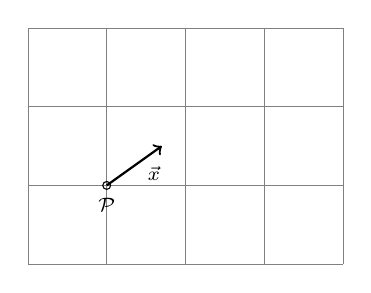
\begin{tikzpicture}
        \draw[step=1cm,gray,very thin] (0,0) grid (4,3);
        \node at (1,0.75) {\scriptsize $\mathcal{P}$};
        \draw (1,1) circle (0.05);
        \node at (1.6,1.15) {\scriptsize $\vec{x}$};
        \draw[thick,->] (1,1) -- (1.7,1.5);
    \end{tikzpicture}
    \caption{A small displacement from $\mathcal{P}$.} \label{fig:vector-displacement}
\end{figure}

The position of a point on the tabletop (Figure \ref{fig:vector-displacement}) is given by a position vector and the temperature by the function $T$. We start at the point $\mathcal{P}$, reached by the position vector $\vec{p}$, where the temperature is $T(\vec{p})$, and we want to know by how much the temperature will change if we move by a small displacement $\vec{x}$.

The answer is given by the function $dT(\vec{x})$, which will be a different function depending on where $\mathcal{P}$ is. We can sort of cheat and define it in terms of $T$ with perfect accuracy:

$$
dT(\vec{x}) = T(\vec{p} + \vec{x}) - T(\vec{p})
$$

But that would be overkill. All we really need is a linear approximation that is only precisely accurate at $\mathcal{P}$, where it has the value zero, but will change linearly with increasing distance (and may diverge from the truth). 

That is, for any scalar constant $k$:

$$
dT(k \vec{x}) = k \, dT(\vec{x})
$$

As $k$ shrinks, the error vanishes:

\begin{equation}
    dT(\vec{x}) = \lim_{k \to 0} \frac{T(\vec{p} + k\vec{x}) - T(\vec{p})}{k}
    \label{eqn:directional-derivative-limit}
\end{equation}

Having chosen a direction, the $dT$ function's value will be proportional to the distance moved, which is to say, the magnitude of the supplied displacement vector. The smaller the displacement, the smaller the value, but also the smaller the error. For large displacement it may be wildly wrong; it doesn't carry enough information about the shape of the temperature map contained in $T$ to reproduce it perfectly. It only knows something about how $T$ changes in the immediate vicinity of $\mathcal{P}$, but that's enough, because if $T$ is a complicated function then there will be a different $dT$ function associated with each point in space, and that variation will encode the underlying shape of $T$.

A function that maps vectors to scalars in this simple linear way is clearly a covector, $\vec{d}$. Given a covector basis $\vec{e}^n$, there will be a set of coordinates $d_n$:

\begin{equation}
    dT(\vec{x}) = \vec{d} = \sum_n \vec{e}^n d_n
    \label{eqn:covector-directional-derivative}
\end{equation}

For every covector there is a dual vector, from the vector space that we use to describe the displacement $x$, that we could use to convey the same information as $\vec{d}$. If we call that vector $\vec{s}$ (short for "slope", for reasons that may become clear), we know how to convert covector coordinates into vector coordinates with the inverse metric $g^{\mu\nu}$:

\begin{equation}
\begin{split}
\vec{s} 
&= \sum_{\mu} \left( \sum_{\nu} g^{\mu\nu} d_{\nu} \right) \vec{e}_{\mu} \\
&= \sum_{\mu} s_{\mu} \vec{e}_{\mu}
\label{eqn:vector-gradient}
\end{split}
\end{equation}

Of course just as the function $df$ (a.k.a. the covector $\vec{d}$) is different at each point in the physical space, so too is the corresponding vector $\vec{s}$. It's a vector field. The official name for $\vec{s}$ is the \textit{gradient}\footnote{We can't reasonably call it $\vec{g}$, as that is the metric (blame Gauss.)} of $T(x)$.

\subsection{Uniform gradient in orthonormal basis}

\begin{figure}[h]
    \caption{Simplified scalar field}
    \centering
    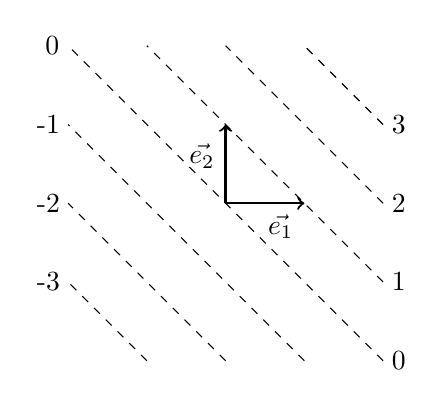
\begin{tikzpicture}
        \draw[dashed] (1,0) -- (0,1);
        \node at (-0.25,1) {-3};
        \draw[dashed] (2,0) -- (0,2);
        \node at (-0.25,2) {-2};
        \draw[dashed] (3,0) -- (0,3);
        \node at (-0.25,3) {-1};
        \draw[dashed] (4,0) -- (0,4);
        \node at (-0.2,4) {0};
        \node at (4.2,0) {0};
        \draw[dashed] (4,1) -- (1,4);
        \node at (4.2,1) {1};
        \draw[dashed] (4,2) -- (2,4);
        \node at (4.2,2) {2};
        \draw[dashed] (4,3) -- (3,4);
        \node at (4.2,3) {3};
        \draw[thick,->] (2,2) -- (3,2);
        \node at (2.7,1.7) {$\vec{e_1}$};
        \draw[thick,->] (2,2) -- (2,3);
        \node at (1.7,2.6) {$\vec{e_2}$};
    \end{tikzpicture}
    \label{fig:scalar-field-std-basis}
\end{figure}

To drastically simplify, we'll consider a scalar field that has the same gradient everywhere in space. This means that the temperature function of absolute position $T(\vec{p})$ depends in a simple way on the position. We can define it in familiar way by using the standard basis, that is, orthonormal basis vectors $\vec{e}_n$, which are shown in Figure \ref{fig:scalar-field-std-basis} overlaid on dashed lines of equal temperature.

The temperature as a function of the position coordinates $p^n$ is given by:

\begin{equation}
    T(\vec{p}) = p^1 + p^2
    \label{eqn:t-absolute}
\end{equation}

The temperature is simply the sum of the coordinates, and so at the origin the temperature is $0$, likewise at coordinates $(1, -1), (2, -2), (-1, 1), (-2, 2)$ and so on, which is to say that there is a diagonal line along which $T$ is $0$. Similarly there is a parallel line along which $T$ is $1$, another where it is $-1$ and so on. These lines are \textit{isolines} or \textit{contours}\footnote{Strangely they are sometimes called "contour lines" even if they are curved paths. The word "line" was once used to refer to any path, curved or straight, and this usage survives in some terminology.}

The simplification arsing from a scalar field whose contours are evenly spaced parallel lines is that although $T$ changes with position, there is no variation in \textit{how it changes} with position. This means that the function $dT$ for the change made by a small displacement $\vec{x}$ is structurally identical to \eqref{eqn:t-absolute}:

\begin{equation}
    dT(\vec{x}) = x^1 + x^2
    \label{eqn:t-rel}
\end{equation}

(As always in this topic, $x^2$ means the second coordinate of a column vector, not the square of a variable $x$.) We can express this function in matrix multiplication:

\begin{equation}
    T(\vec{x}) = 
    \begin{bmatrix}1 & 1\end{bmatrix}
    \begin{bmatrix}x^1 \\ x^2\end{bmatrix}
    \label{eqn:t-rel-matrices}
\end{equation}

That is, it's the action of a covector with coordinates $(1, 1)$, which we called $\vec{d}$ in \eqref{eqn:covector-directional-derivative}:

$$
T(\vec{x}) = \langle \vec{d}, \vec{x} \rangle
$$

The dual of $\vec{d}$ is the vector we called $\vec{s}$ in \eqref{eqn:vector-gradient}, and because we're in the standard orthonormal basis the coordinates are the same, $d_n = s^n$. This is the gradient vector and can be legitimately drawn in physical space as a vector (Figure \ref{fig:gradient-vector}).

\begin{figure}[h]
    \caption{Gradient vector}
    \centering
    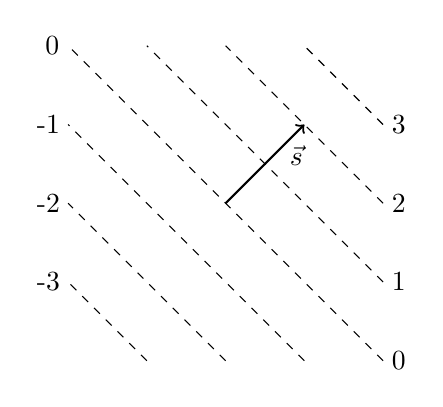
\begin{tikzpicture}
        \draw[dashed] (1,0) -- (0,1);
        \node at (-0.25,1) {-3};
        \draw[dashed] (2,0) -- (0,2);
        \node at (-0.25,2) {-2};
        \draw[dashed] (3,0) -- (0,3);
        \node at (-0.25,3) {-1};
        \draw[dashed] (4,0) -- (0,4);
        \node at (-0.2,4) {0};
        \node at (4.2,0) {0};
        \draw[dashed] (4,1) -- (1,4);
        \node at (4.2,1) {1};
        \draw[dashed] (4,2) -- (2,4);
        \node at (4.2,2) {2};
        \draw[dashed] (4,3) -- (3,4);
        \node at (4.2,3) {3};
        \draw[thick,->] (2,2) -- (3,3);
        \node at (2.9,2.6) {$\vec{s}$};
    \end{tikzpicture}
    \label{fig:gradient-vector}
\end{figure}

Note how it is perpendicular to the contours. It points in the direction of "steepest increase" of the field. Also its magnitude is significant: if you move $1$ unit of distance along the direction of $\vec{s}$, the field will increase by $\|\vec{s}\|$, which in this case is $\sqrt{2}$.

(The diagram is possibly confusing on this point, because it actually shows that a displacement by $\vec{s}$, i.e. moving along the direction of $\vec{s}$ by distance $\|\vec{s}\|$, will increase $T$ by $2$, which is the same thing.)

\subsection{Uniform gradient in a non-orthonormal basis}

How can we be sure that this description wasn't affected by our use of the standard basis?

\begin{figure}[h]
    \caption{Simplified scalar field in another basis}
    \centering
    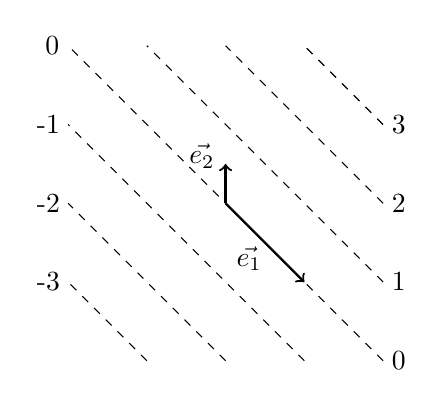
\begin{tikzpicture}
        \draw[dashed] (1,0) -- (0,1);
        \node at (-0.25,1) {-3};
        \draw[dashed] (2,0) -- (0,2);
        \node at (-0.25,2) {-2};
        \draw[dashed] (3,0) -- (0,3);
        \node at (-0.25,3) {-1};
        \draw[dashed] (4,0) -- (0,4);
        \node at (-0.2,4) {0};
        \node at (4.2,0) {0};
        \draw[dashed] (4,1) -- (1,4);
        \node at (4.2,1) {1};
        \draw[dashed] (4,2) -- (2,4);
        \node at (4.2,2) {2};
        \draw[dashed] (4,3) -- (3,4);
        \node at (4.2,3) {3};
        \draw[thick,->] (2,2) -- (3,1);
        \node at (2.3,1.3) {$\vec{e_1}$};
        \draw[thick,->] (2,2) -- (2,2.5);
        \node at (1.7,2.6) {$\vec{e_2}$};
    \end{tikzpicture}
    \label{fig:scalar-field-awkward-basis}
\end{figure}

Let's rewind back to the start and pick a different basis (Figure \ref{fig:scalar-field-awkward-basis}). We've changed $\vec{e}_1$ to point diagonally downwards and to the right, so in terms of the standard basis it would have coordinates $(1, -1)$. We've also made $\vec{e}_2$ half its previous length.

The significant thing about this (apart from the abandoning of both orthogonality and equal lengths) is that $\vec{e}_1$ is parallel to the contours. This means that a displacement that adjusts only the first coordinate will not affect the value of $T$, because it just moves along the current contour. But a displacement in the second coordinate will have half the effect it had before. So we expect:

\begin{equation}
    dT(\vec{x}) = \frac{1}{2}x^2
    \label{eqn:t-rel-awk}
\end{equation}

(Again, that is not "x squared"! It's the second coordinate of $\vec{x}$.) Or in matrix multiplication it's:

\begin{equation}
    T(\vec{x}) = 
    \begin{bmatrix}0 & \frac{1}{2}\end{bmatrix}
    \begin{bmatrix}x^1 \\ x^2\end{bmatrix}
    \label{eqn:t-rel-matrices-awk}
\end{equation}

That is, it's the action of a covector $\vec{d}$ with coordinates $(0, \frac{1}{2})$:

$$
T(\vec{x}) = \langle \vec{d}, \vec{x} \rangle
$$

As always, a covector $\vec{d}$ must have a dual vector $\vec{s}$, but this time we can't simply transpose the row of coordinates $d_n$ into a column of $s^n$. The coordinates of the dual vector/covector pair are different in a non-orthonormal basis. We can use the inverse metric (the "raising" metric) to convert the coordinates, if we can figure out what it is. The shortcut is to express our basis vectors as coordinates in terms of the standard orthonormal basis:

$$
\vec{e}_1 = \begin{bmatrix}
    1 \\
    -1
\end{bmatrix}
\, , \,
\vec{e}_2 = \begin{bmatrix}
    0 \\
    \frac{1}{2}
\end{bmatrix}
$$

and then the lowering metric's elements can be calculated by the dot product\footnote{This is only allowed because we're temporarily back in the standard orthonormal basis!}:

\begin{equation}
\begin{split}
    g_{\mu\nu} &= \vec{e}_{\mu} \cdot \vec{e}_{\nu} \\
    &= \begin{bmatrix}
        2 & -\frac{1}{2} \\
        -\frac{1}{2} & \frac{1}{4}
        \end{bmatrix}
\end{split}
\end{equation}

The raising metric is the inverse of that:

\begin{equation}
    g^{\mu\nu} = 
    \begin{bmatrix}
    1 & 2 \\
    2 & 8
    \end{bmatrix}
\end{equation}

So we can apply that to our transposed $d_n$ coordinates to get $s^n$ coordinates:

$$
\begin{bmatrix}
    1 & 2 \\
    2 & 8
\end{bmatrix}
\begin{bmatrix}
    0 \\
    \frac{1}{2}
\end{bmatrix}
= 
\begin{bmatrix}
    1 \\
    4
\end{bmatrix}
$$

And once again, these being the coordinates of an ordinary vector, we can legitimately plot that vector on the same diagram of the field's contours:

\begin{figure}[h]
    \caption{Gradient vector in other basis}
    \centering
    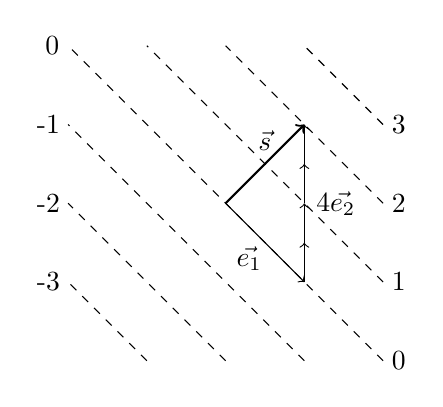
\begin{tikzpicture}
        \draw[dashed] (1,0) -- (0,1);
        \node at (-0.25,1) {-3};
        \draw[dashed] (2,0) -- (0,2);
        \node at (-0.25,2) {-2};
        \draw[dashed] (3,0) -- (0,3);
        \node at (-0.25,3) {-1};
        \draw[dashed] (4,0) -- (0,4);
        \node at (-0.2,4) {0};
        \node at (4.2,0) {0};
        \draw[dashed] (4,1) -- (1,4);
        \node at (4.2,1) {1};
        \draw[dashed] (4,2) -- (2,4);
        \node at (4.2,2) {2};
        \draw[dashed] (4,3) -- (3,4);
        \node at (4.2,3) {3};
        \draw[thick,->] (2,2) -- (3,3);
        \node at (2.5,2.8) {$\vec{s}$};
        \draw[thin,->] (2,2) -- (3,1);
        \node at (2.3,1.3) {$\vec{e_1}$};
        \draw[thin,->] (3,1) -- (3,1.5);
        \draw[thin,->] (3,1.5) -- (3,2);
        \draw[thin,->] (3,2) -- (3,2.5);
        \draw[thin,->] (3,2.5) -- (3,3);
        \node at (3.4,2) {$4\vec{e_2}$};
    \end{tikzpicture}
    \label{fig:gradient-vector-awk}
\end{figure}

For absolute clarity we've spelled out the scaling and addition of the basis vectors, to show that $\vec{s}$ is equivalent to adding $4$ lots of $\vec{e}_2$ on to the end of $\vec{e}_1$, just as the coordinates of $\vec{s}$ tell us to do. But the key point is that this is physically the same vector we found when working in the standard orthonormal basis (Figure \ref{fig:gradient-vector}). It is described by different coordinates, of course, but it's the same vector, pointing in the direction of steepest increase. It even has the same magnitude $\|\vec{s}\|$, which is the square root of the inner product of $\vec{s}$ with itself. The inner product will use the lowering metric to convert one of those $\vec{s}$ inputs to $\vec{d}$ so it can act on the other $\vec{s}$, ensuring a consistent result.

Similarly, given $\vec{s}$ and some other vector $\vec{x}$ representing a displacement, we can directly obtain the change in $T$ due to that displacement using the inner product $(\vec{s}, \vec{x})$ between them:

\begin{equation}
\begin{split}
dT &= (\vec{s}, \vec{x}) \\
   &= \sum_{\nu} \left( \sum_{\mu} g_{\mu\nu} s^{\mu} \right) x^{\nu} \\
    &= \sum_{\nu} d_{\nu} x^{\nu}
\end{split}
\end{equation}

\subsection{Smoothly varying gradients}

Generalising this to the more complicated kinds of $T$ scalar field, the scalar-valued function $dT(\vec{x})$, which tells us how $T$ changes due to a small displacement $\vec{x}$, may have a different definition at each point in space. But we can retain the simplification that we only need to know the linear approximation of that function at each point.

The displacement will be described by a number in each dimension: a relative coordinate change associated with each position basis vector. If we only allow one coordinate, $x^i$, to vary and leave the others constant, $dT$ becomes a scalar-valued function of a single variable, $x^i$, which if plotted would simply be a line through the origin (i.e. it is $0$ when its parameter is $0$). It is therefore characterised entirely by a single number, its gradient, the number by which it multiplies its input.

The function $T$ is of course not necessarily linear in $x^i$. Following the Maclaurin method (§\ref{sec:unit-circle-maclaurin}), we assume that whatever the function is, it can be expressed as a polynomial series\footnote{Warning! In this context we're dealing with scalar variables and $x^n$ briefly means "$x$ to the power of $n$", not the $n$th component of $\vec{x}$.} of the form $d_n x^n$. The first term ($n = 0$, $x^0 = 1$) is just a constant: the value of $T$ at the current position. We will be subtracting this from the total, because we want to know how $T$ changes as we move away from that position. The terms $n > 1$ involve $x^2$, $x^3$ and so on. As $x$ becomes arbitrarily small, these terms plummet in significance very rapidly. So that leaves just the term $d_1 x$, and $d_1$ is the only number we need to describe the tangent line to the curve of the function at the current position. We can therefore discard its subscript label, and replace it with $i$, as it's the sole outcome of this analysis when varying the $i$th component of $\vec{x}$:

$$
\frac{\partial T(\vec{x})}{\partial x^i} = d_i
$$

We carry out this analysis $i$ times to get the linear gradient number for all $i$ components, and thanks to linearity we can simply add them to get the total change in $F$:

$$
d T(\vec{x}) = \sum_i \frac{\partial T(\vec{x})}{\partial x^i}
= \sum_i d_i x^i
= \langle \vec{d} , \vec{x} \rangle
$$

Once again it's just the covector $\vec{d}$ described by coordinates $d_i$, acting on the displacement vector $\vec{x}$ described by coordinates $x^i$. Then to obtain the components of the gradient vector, which is the dual of $d$, we apply the raising metric $g^{\mu\nu}$ to $d$.

The trivial example of the linear field with constant gradient $T(\vec{x}) = x^1 + x^2$ was therefore in fact fully illustrative, because if the function had any terms that weren't linear, we would have just ignored them anyway.

\subsection{Sources of confusion}

A major potential source of confusion in this area is the distinction between the total derivative, a covector, and the gradient, a vector, and how and why they might be affected by a change of basis. As we've seen, they are \textit{not} affected by a change of basis. Vectors and covectors never are. Their coordinates are affected, of course.

Another source of confusion is the way we think of the gradient as the rate of change of the scalar field, computed with respect to a change in position. This means that a physical distance appears on the bottom of a fraction, and therefore if we increase the size of our unit of distance, the number on the bottom of the fraction decreases, which increases the overall value of the fraction. This reminds us of covariance; is this the source of some inherently covector-like nature in gradients? No. As we've seen, the gradient is actually a vector, and so its coordinates transform contravariantly. The total derivative is a covector that maps a displacement vector to a change in the scalar field, so its coordinates transform covariantly. These two representations actually convey the same information (even in the form of the same set of numbers if the basis is orthonormal), so there is nothing inherently covariant about that information.

\section{Complex vector spaces}\label{sec:vectors-complex}

We've mentioned that a vector space has an associated set of scalars, and this is often $\mathbb{R}$, but it may instead be $\mathbb{C}$, meaning that vectors can be scaled by a complex number, and if expressed as a column of coordinates, those coordinates may be complex.

Even the simplest non-trivial example of such a space, $\mathbb{C}^2$, is not directly imaginable, because although each vector requires two coordinates, each of those is a complex number incorporating a real and imaginary part, so each vector requires four real numbers to describe it, and so $\mathbb{C}^2$ is isomorphic with $\mathbb{R}^4$, which is impossible to visualise directly.

Even so, concepts applicable to real vector spaces also work for complex, although with some modifications. Linear independence of a set of N vectors still means that no one of them can be recreated via a linear combination of the others. A mapping from a vector to a scalar, where the scalar is a complex number, is still called a covector. All the related concepts work the same.

\subsection{Complex dual space}

A basis of linearly independent vectors can be chosen, and a dual basis in the covectors is then defined by \eqref{eqn:dual-bases-delta}:

$$
\langle \vec{e}^i,\vec{e}_j\rangle = \delta\indices{^i_j}
$$  

For example, regarding column vectors from $\mathbb{C}^2$, these are linearly independent:

$$
\vec{e}_1 = \begin{bmatrix}1 \\ 0\end{bmatrix}
, \,
\vec{e}_2 = \begin{bmatrix}0 \\ i\end{bmatrix}
$$

We gleaned from our experiments with one-hot basis vectors in $\mathbb{R}^2$ that $\vec{e}^1 = \begin{bmatrix}1 & 0\end{bmatrix}$, to ensure that $\langle \vec{e}^1,\vec{e}_1\rangle = 1$. By leaning on our schoolhouse assumption of orthonormality based on the dot product, we observed that if the basis vectors are orthonormal, each basis covector will have the same coordinates as its corresponding basis vector.

But by definition $(i)^2 = -1$. So to ensure $\langle \vec{e}^2,\vec{e}_2\rangle = 1$, it must be that:

$$
\vec{e}^2 = \begin{bmatrix}0 & -i\end{bmatrix}
$$

Intriguing! What $1$ and $i$ have in common is that they are unitary (having modulus $1$). On the complex plane such numbers form the unit circle $e^{i\theta}$ (§\ref{euler-formula}). When $\theta = \pi / 4$ (45\textdegree) the real and imaginary ingredients are balanced, making an equal contribution to it having modulus $1$:

$$
\frac{1}{\sqrt{2}} + \frac{i}{\sqrt{2}}
$$

Both terms squared equal a half, so Pythagoras finds the "length" of the number to be $1$. An equivalent way to find the modulus is to multiply the number by its complex conjugate, where the sign of the imaginary part is reversed. So if:

$$
\vec{e}_2 = \begin{bmatrix}0 \\ \frac{1}{\sqrt{2}} + \frac{i}{\sqrt{2}}\end{bmatrix}
$$

then it must be that:

$$
\vec{e}^2 = \begin{bmatrix}0 \\ \frac{1}{\sqrt{2}} - \frac{i}{\sqrt{2}}\end{bmatrix}
$$

The covector coordinates are not the same: they are the conjugates of the vector coordinates. Of course, a real number having zero imaginary part, it is equal to its own conjugate, which is why our original "same coordinates" rule worked. But we have now shown how to amend it to cover complex vector spaces in a backward compatible way.

In matrix terms, a covector acts on a vector by a row multiplying with a column. By selecting an orthonormal basis according to whatever inner product exists, the inner product expressed in that basis becomes the dot product, so a vector is able to "act on" any other vector just like it was a covector. A vector can act on itself with the dot product to find its own norm-squared. But we generally expect the norm of a vector to be a positive real number, even though the vector may have complex components.

So given two vectors $\vec{a}$ and $\vec{b}$ defined by column matrices $a$ and $b$, where before the simple form of the inner product was defined as:

$$
(\vec{a}, \vec{b}) = (a^\intercal) b = a_n b_n
$$

it is now given by:

$$
(\vec{a}, \vec{b}) = (a^\dagger) b = (a_n^*) b_n
$$

where we use the dagger $^\dagger$ symbol to mean \textit{conjugate transpose}, where we both transpose the matrix and also take the complex conjugate of every element. This is also called the \textit{Hermitian transpose}.

Care has been taken above to use parentheses to clarify that $^\dagger$ and $^*$ are operators acting on the single object to their left, but these are usually omitted:

$$
(\vec{a}, \vec{b}) = a^\dagger b = a_n^* b_n
$$

This might be misconstrued as suggesting that $^\dagger$ is a binary operator acting on the two objects on either side of it, like $+$, so be wary.

Although this definition ensures the norm is positive and real, it has the downside of destroying the symmetry of the inner product between two different vectors:

$$
(\vec{a}, \vec{b})
\ne
(\vec{b}, \vec{a})
$$

All we can say is that:

$$
(\vec{a}, \vec{b})
=
\left[ (\vec{b}, \vec{a}) \right]^*
$$

This is sometimes called conjugate symmetry. This does mean that when taking the inner product of two different complex vectors, it matters to which one we apply the dagger. In physics the convention is to take the conjugate of the left vector, as shown above, and in pure mathematics they take the conjugate of the right vector - \textit{c'est la vie}.

\subsection{Hermitian operators}

A similar adjustment must be made to the idea of a symmetric matrix (§\ref{ch:vectors-symmetric}), with their useful properties. Rather than requiring the matrix to equal its own transpose, it must equal its own Hermitian transpose:

$$M^\dagger = M$$

That is, every element is the complex conjugate of its diagonally opposing element:

$$M_{ij} = (M_{ji})^*$$

Therefore elements on the diagonal are real (they aren't moved by the transposition and so must equal their own complex conjugates). We call this a Hermitian matrix.

Regardless of the basis, given an inner product, if:

$$(\hat{M} \vec{a}, \vec{b}) = (\vec{a}, \hat{M} \vec{b})$$

then $\hat{M}$ is a Hermitian operator, and in an orthogonal basis it is represented by a Hermitian matrix.

Several other important facts about Hermitian operators can be derived: their eigenvalues are all real and from their eigenvectors it is possible to choose an orthonormal basis that spans the space.

\subsection{Complex unitary operators}

We defined unitary operators in real spaces by saying that their inverse is their transpose. Unsurprisingly in complex spaces this definition has to be modified:

$$(O^\dagger) O = I$$

Also the intuitive understanding that a unitary operator performs a combination of rotation and reflection on a vector is no longer strictly true, because it may also "rotate" the individual coordinates in the complex plane (that is, multiply them by a unitary complex number).